% ---------------------------------------------------------------------------
% dendritic_credit_workshop_25.tex — 26-slide workshop rebuild.
%
% Single-deck build (pdflatex only): core slides + Backup divider + backup
% frames in ONE PDF —
%   pdflatex dendritic_credit_workshop_25.tex
%
% Visual system: white ground, TeX Gyre Heros text, CM italic math,
% journal CVD-validated palette. Do not repurpose hues against their
% semantic roles (green=shunting/anatomy-route, blue=additive,
% red-brown=backprop ceiling, amber=scalar/local, violet=oracle,
% gray=point/control).
% ---------------------------------------------------------------------------
\documentclass[aspectratio=169,10pt]{beamer}

\usepackage[T1]{fontenc}
\usepackage[utf8]{inputenc}
\usepackage{tgheros}
\renewcommand{\familydefault}{\sfdefault}
\usepackage{amsmath,amssymb,bm,mathtools,booktabs,array,etoolbox}
\usepackage{graphicx}
\usepackage{tikz}
\usetikzlibrary{arrows.meta,calc,positioning,shapes.geometric,decorations.pathreplacing,fit,backgrounds}
\pdfstringdefDisableCommands{\def\translate#1{#1}}
\hypersetup{pdftitle={When dendritic structure helps local credit assignment},
            pdfauthor={Safaai, Richards, Sabatini}}

% ---- palette (journal CVD-validated system) -------------------------------
\definecolor{Ink}{HTML}{232323}       % primary text
\definecolor{Mute}{HTML}{69707A}      % secondary text / scaffolding
\definecolor{Grid}{HTML}{E3E7EC}      % hairlines
\definecolor{Paper}{HTML}{F7F8FA}     % pale panels
\definecolor{Shunt}{HTML}{3FA26C}     % shunting / anatomy-route
\definecolor{ShuntPale}{HTML}{E5F2EB}
\definecolor{Add}{HTML}{20509E}       % additive
\definecolor{AddPale}{HTML}{E8EFF9}
\definecolor{BP}{HTML}{932F1E}        % backprop / exact ceiling
\definecolor{Amber}{HTML}{E2A23F}     % scalar / local
\definecolor{Violet}{HTML}{8F66CD}    % oracle
\definecolor{Rose}{HTML}{E28FBC}
\definecolor{Soma}{HTML}{E8873C}
\definecolor{Dend}{HTML}{3E8E63}
\definecolor{Exc}{HTML}{2C6CB0}
\definecolor{Inh}{HTML}{B13138}

% ---- beamer chrome --------------------------------------------------------
\setbeamercolor{normal text}{fg=Ink,bg=white}
\setbeamercolor{frametitle}{fg=Ink,bg=white}
\setbeamercolor{structure}{fg=Shunt}
\setbeamercolor{alerted text}{fg=BP}
\setbeamercolor{footline}{fg=Mute,bg=white}
\setbeamercolor{claimpanel}{fg=Ink,bg=Paper}
\setbeamertemplate{navigation symbols}{}
\setbeamertemplate{headline}{}
\setbeamertemplate{itemize item}{\color{Shunt}\scriptsize\raisebox{0.12ex}{$\bullet$}}
\setbeamertemplate{itemize subitem}{\color{Mute}\tiny\raisebox{0.18ex}{$\bullet$}}
\setbeamersize{text margin left=0.7cm,text margin right=0.7cm}

% ---- core-slide accounting ------------------------------------------------
\newcommand{\CoreSlides}{26}

% ---- frame title: bold Heros claim, optional Mute subtitle, Grid hairline -
\setbeamertemplate{frametitle}{%
  \vspace{0.52cm}%
  {\fontsize{14}{16.8}\selectfont\bfseries\color{Ink}\insertframetitle\par}%
  \ifx\insertframesubtitle\empty\else
    \vspace{0.10cm}%
    {\fontsize{9}{11}\selectfont\color{Mute}\insertframesubtitle\par}%
  \fi
  \vspace{0.16cm}%
  {\color{Grid}\rule{\textwidth}{0.35pt}\par}%
  \vspace{0.12cm}%
}

% ---- footline: single hairline-free line ----------------------------------
\setbeamertemplate{footline}{%
  \leavevmode\hbox{%
    \begin{beamercolorbox}[wd=0.72\paperwidth,ht=0.30cm,dp=0.14cm,leftskip=0.7cm]{footline}%
      \color{Mute}\tiny Dendritic credit\enspace\textperiodcentered\enspace Kempner Learning Dynamics 2026%
    \end{beamercolorbox}%
    \begin{beamercolorbox}[wd=0.28\paperwidth,ht=0.30cm,dp=0.14cm,rightskip=0.7cm]{footline}%
      \hfill\color{Mute}\tiny\insertframenumber\,/\,\CoreSlides%
    \end{beamercolorbox}}%
}

% ===========================================================================
% Shared TikZ schematic vocabulary (matches the journal figures)
% ===========================================================================
\tikzset{
  dendarrow/.style={-{Stealth[length=4pt]},line width=0.9pt},
  scaffold/.style={Mute,line width=0.5pt,dash pattern=on 1.6pt off 1.4pt},
  junction/.style={circle,draw=Dend,fill=white,line width=0.6pt,inner sep=0pt,minimum size=3.2pt},
}

% Credit-tree schematic library: \CreditTree (modes forward/eligibility/
% transport/scalar/coordinate/address/gain/shunt), \DerangedPair,
% \TreeStrip, \eqpanel, \triptych, \deftag. Regression page:
% credit_tree_lib_test.tex.
% ---------------------------------------------------------------------------
% credit_tree_lib.tex — THE CREDIT-TREE SCHEMATIC LIBRARY.
%
% One parameterized dendritic tree, drawn with identical geometry on every
% slide; only its DECORATION changes to show the quantity being defined or
% manipulated. Load from the workshop preamble via % ---------------------------------------------------------------------------
% credit_tree_lib.tex — THE CREDIT-TREE SCHEMATIC LIBRARY.
%
% One parameterized dendritic tree, drawn with identical geometry on every
% slide; only its DECORATION changes to show the quantity being defined or
% manipulated. Load from the workshop preamble via % ---------------------------------------------------------------------------
% credit_tree_lib.tex — THE CREDIT-TREE SCHEMATIC LIBRARY.
%
% One parameterized dendritic tree, drawn with identical geometry on every
% slide; only its DECORATION changes to show the quantity being defined or
% manipulated. Load from the workshop preamble via \input{credit_tree_lib.tex}
% (after the palette definitions and \usetikzlibrary lines).
%
% Public interface
%   \CreditTree[mode=<m>, scale=<s>, stagelabel=<text>, K=<2|4|8>,
%               shunted=<true|false>]
%     modes: plain | forward | eligibility | transport | scalar | coordinate |
%            address (uses K) | gain | shunt (uses shunted)
%     plain is the notation-free hook variant: tree, soma, synapse dots and
%     an unlabeled arriving-error arrow — no algebra labels.
%   \DerangedPair[<scale>]        correct vs deranged coordinate assignment
%   \TreeStrip{<stage1>}{<stage2>}...   2-4 stages, Mute arrows between
%       (scans for further brace groups; end with \par/newline or \relax
%        before any unrelated literal `{`)
%   \eqpanel[<TAG>]{<equations>}  Paper card, hairline border, Mute eyebrow
%   \triptych{<left>}{<middle>}{<right>}  0.30/0.30/0.36 top-aligned columns
%   \deftag{<word>}               inline definition eyebrow
%
% All trees share the SAME coordinates so cross-slide changes read as the
% same object. tikzpicture baseline is pinned at the soma center (0,0), so
% side-by-side trees align on their somas regardless of decorations.
% Node fonts do not scale with [scale=...]; keep scale in 0.5-1.4.
% ---------------------------------------------------------------------------

% ---- keys -----------------------------------------------------------------
\pgfkeys{
  /credittree/.is family, /credittree,
  mode/.store in       = \ctmode,
  scale/.store in      = \ctscale,
  stagelabel/.store in = \ctstagelabel,
  K/.store in          = \ctK,
  shunted/.store in    = \ctshunted,
  default keys/.style  = {mode=forward, scale=1, stagelabel={}, K=4,
                          shunted=true},
}

% ---- shared styles ----------------------------------------------------------
\tikzset{
  ctjunction/.style={circle,draw=Dend,fill=white,line width=0.6pt,
                     inner sep=0pt,minimum size=3.2pt},
  ctsyn/.style={circle,inner sep=0pt,minimum size=3.6pt},
  ctlab/.style={font=\scriptsize,inner sep=1pt},
  cttiny/.style={font=\tiny,inner sep=1pt},
  ctfield/.style={font=\scriptsize,inner sep=1pt},
}

% ---- fixed geometry (identical across ALL modes) ----------------------------
\newcommand{\CTcoordinates}{%
  \coordinate (S)   at ( 0.00,0.00);
  \coordinate (J1)  at ( 0.06,0.85);
  \coordinate (JL)  at (-0.92,1.52);
  \coordinate (JR)  at ( 0.88,1.44);
  \coordinate (JLL) at (-1.72,2.02);
  \coordinate (JLR) at (-0.58,2.32);
  \coordinate (JRL) at ( 0.56,2.28);
  \coordinate (JRR) at ( 1.62,1.92);
  \coordinate (T1)  at (-2.30,2.42);
  \coordinate (T2)  at (-1.52,2.82);
  \coordinate (T3)  at (-0.92,3.02);
  \coordinate (T4)  at (-0.22,3.06);
  \coordinate (T5)  at ( 0.28,3.04);
  \coordinate (T6)  at ( 0.94,2.94);
  \coordinate (T7)  at ( 1.54,2.72);
  \coordinate (T8)  at ( 2.24,2.28);
}

% Stroke taper (pt at scale 1): trunk / level-2 / level-3 / terminal.
% \ctlwf tempers line widths and capsule widths at small scales.
\newcommand{\CTsetwidths}{%
  \pgfmathsetmacro{\ctlwf}{min(1.15,max(0.62,\ctscale))}%
  \pgfmathsetmacro{\cttmp}{1.60*\ctlwf}\edef\ctwA{\cttmp pt}%
  \pgfmathsetmacro{\cttmp}{1.20*\ctlwf}\edef\ctwB{\cttmp pt}%
  \pgfmathsetmacro{\cttmp}{0.90*\ctlwf}\edef\ctwC{\cttmp pt}%
  \pgfmathsetmacro{\cttmp}{0.70*\ctlwf}\edef\ctwD{\cttmp pt}%
}

% Whole tapered tree in one style (color / opacity list in #1).
\newcommand{\CTplaintree}[1]{%
  \draw[#1,line width=\ctwA] (0,0.17) -- (J1);
  \draw[#1,line width=\ctwB] (J1) -- (JL)  (J1) -- (JR);
  \draw[#1,line width=\ctwC] (JL) -- (JLL) (JL) -- (JLR)
                             (JR) -- (JRL) (JR) -- (JRR);
  \draw[#1,line width=\ctwD] (JLL) -- (T1) (JLL) -- (T2)
                             (JLR) -- (T3) (JLR) -- (T4)
                             (JRL) -- (T5) (JRL) -- (T6)
                             (JRR) -- (T7) (JRR) -- (T8);
}

\newcommand{\CTjunctions}[1]{%
  \foreach \ctj in {J1,JL,JR,JLL,JLR,JRL,JRR}
    \node[ctjunction,#1] at (\ctj) {};
}

% #1 = fill, #2 = draw
\newcommand{\CTsoma}[2]{%
  \filldraw[fill=#1,draw=#2,line width=0.6pt] (0,0) circle (0.185);
}

\newcommand{\CTstagelabel}{%
  \ifdefempty{\ctstagelabel}{}{%
    \node[anchor=north,font=\scriptsize,text=Mute] at (0,-0.30)
      {\ctstagelabel};}%
}

% Route-field capsule: pale SOLID tints (translucent look, no PDF
% transparency, so overlaps never double-darken).  #1 tint, #2 width factor,
% #3 path.
\newcommand{\CTcapsule}[3]{%
  \pgfmathsetmacro{\cttmp}{#2*\ctlwf}%
  \draw[#1,line width=\cttmp pt,line cap=round,line join=round] #3;
}

% ===========================================================================
% \CreditTree
% ===========================================================================
\newcommand{\CreditTree}[1][]{%
  \pgfkeys{/credittree, default keys, #1}%
  \begin{tikzpicture}[scale=\ctscale,line cap=round,baseline={(0,0)}]
    \CTsetwidths
    \CTcoordinates
    % ------------------------------------------------------------ plain ----
    % Hook variant: the anatomy and its synapses, no notation. Used before
    % any forward-model vocabulary is defined (deck slide 2).
    \ifdefstring{\ctmode}{plain}{%
      \CTplaintree{Dend}
      \CTjunctions{}
      \CTsoma{Soma}{Ink!30}
      % synapse population: excitatory dots on the terminal segments
      \foreach \cta/\ctb/\ctf in {JLL/T1/0.55,JLL/T2/0.62,JLR/T3/0.55,
                                  JLR/T4/0.62,JRL/T5/0.55,JRL/T6/0.62,
                                  JRR/T7/0.55,JRR/T8/0.58}
        \node[ctsyn,fill=Exc] at ($(\cta)!\ctf!(\ctb)$) {};
      % two inhibitory contacts near the trunk
      \node[ctsyn,fill=Inh] at ($(J1)!0.55!(JL)$) {};
      \node[ctsyn,fill=Inh] at ($(JR)!0.45!(JRL)$) {};
      % one arriving output error, unlabeled
      \draw[Add,-{Stealth[length=4.5pt]},line width=0.9pt]
        (1.30,0.60) to[bend left=14] (0.27,0.09);
    }{}%
    % ---------------------------------------------------------- forward ----
    \ifdefstring{\ctmode}{forward}{%
      \CTplaintree{Dend}
      \CTjunctions{}
      \CTsoma{Soma}{Ink!30}
      % two example synapses: one excitatory, one inhibitory
      \node[ctsyn,fill=Exc] at ($(JRR)!0.55!(T7)$) {};
      \node[cttiny,anchor=west,text=Exc!60!Ink] at ($(JRR)!0.55!(T7)+(0.12,0.05)$)
        {$g_i,\,E_i$};
      \node[ctsyn,fill=Inh] at ($(J1)!0.55!(JL)$) {};
      \node[cttiny,anchor=east,text=Inh!70!Ink] at ($(J1)!0.55!(JL)+(-0.10,-0.08)$)
        {$g_j,\,E_j$};
      % compartment and soma potentials
      \node[ctlab,anchor=west,text=Ink] at ($(JRR)+(0.20,-0.04)$) {$V_n$};
      \node[ctlab,anchor=west,text=Ink] at (0.26,-0.16) {$V_0$};
      % conductance-quotient anchor: where R_n^tot lives
      \draw[Mute,line width=0.45pt,dash pattern=on 1.4pt off 1.3pt]
        (JRR) -- ++(0.30,-0.62) coordinate (ctq);
      \node[cttiny,anchor=north,text=Mute] at (ctq) {$R_n^{\mathrm{tot}}$};
    }{}%
    % ------------------------------------------------------- eligibility ----
    \ifdefstring{\ctmode}{eligibility}{%
      \CTplaintree{Mute!32}
      % host branch stays alive
      \draw[Dend,line width=\ctwC] (JR) -- (JRL);
      \draw[Dend,line width=\ctwD] (JRL) -- (T6);
      \CTjunctions{draw=Mute!45}
      \node[ctjunction] at (JRL) {};
      \CTsoma{Soma!35}{Ink!15}
      % the synapse under the lens
      \coordinate (ctsynpt) at ($(JRL)!0.55!(T6)$);
      \node[ctsyn,fill=Exc,minimum size=4.6pt,draw=Ink!55,line width=0.5pt]
        at (ctsynpt) {};
      % zoom bubble to the side
      \coordinate (ctzc) at (2.62,1.30);
      \draw[Grid,line width=0.6pt] (ctsynpt) -- ($(ctzc)+(-0.30,0.86)$);
      \draw[Grid,line width=0.6pt] (ctsynpt) -- ($(ctzc)+(-0.88,-0.18)$);
      \filldraw[fill=white,draw=Mute!60,line width=0.7pt] (ctzc) circle (0.92);
      % row 1: presynaptic activity
      \node[ctsyn,fill=Exc] at ($(ctzc)+(-0.52,0.44)$) {};
      \node[ctlab,anchor=west,text=Ink] at ($(ctzc)+(-0.36,0.44)$)
        {$x_i$ \textcolor{Mute}{\tiny presyn.}};
      % row 2: driving-force gauge
      \draw[Mute,line width=0.6pt]
        ($(ctzc)+(-0.52,-0.06)$) ++(200:0.15) arc (200:-20:0.15);
      \draw[Ink,line width=0.7pt]
        ($(ctzc)+(-0.52,-0.06)$) -- ++(52:0.15);
      \node[ctlab,anchor=west,text=Ink] at ($(ctzc)+(-0.30,0.00)$)
        {$E_i-V_n$};
      % row 3: input resistance
      \draw[Ink,line width=0.6pt] ($(ctzc)+(-0.66,-0.50)$)
        -- ++(0.05,0.08) -- ++(0.08,-0.16) -- ++(0.08,0.16)
        -- ++(0.08,-0.16) -- ++(0.05,0.08);
      \node[ctlab,anchor=west,text=Ink] at ($(ctzc)+(-0.28,-0.48)$)
        {$R_n^{\mathrm{tot}}$};
      \node[cttiny,anchor=north,text=Mute] at ($(ctzc)+(0,-0.98)$)
        {local factors of $e_i$};
    }{}%
    % --------------------------------------------------------- transport ----
    \ifdefstring{\ctmode}{transport}{%
      % off-path skeleton, muted
      \CTplaintree{Mute!30}
      \CTjunctions{draw=Mute!40}
      % the traversed root-to-leaf path, additive blue
      \draw[Add,line width=\ctwA] (0,0.17) -- (J1);
      \draw[Add,line width=\ctwB] (J1) -- (JL);
      \draw[Add,line width=\ctwC] (JL) -- (JLR);
      \draw[Add,line width=\ctwD] (JLR) -- (T4);
      % mid-edge arrowheads: credit flows soma -> leaf
      \foreach \cta/\ctb in {{0,0.17}/J1,J1/JL,JL/JLR,JLR/T4}
        \draw[Add,-{Stealth[length=4.5pt]},line width=0.8pt]
          ($(\cta)!0.34!(\ctb)$) -- ($(\cta)!0.60!(\ctb)$);
      % traversed junctions carry their gains
      \foreach \ctj in {J1,JL,JLR} \node[ctjunction,draw=Add] at (\ctj) {};
      \node[ctlab,anchor=west,text=Add] at (0.34,0.66)   {$\alpha_1$};
      \node[ctlab,anchor=east,text=Add] at (-1.16,1.42)  {$\alpha_2$};
      \node[ctlab,anchor=west,text=Add] at (-0.42,2.10)  {$\alpha_3$};
      % soma error and destination
      \CTsoma{Soma}{Ink!30}
      \node[ctlab,anchor=east,text=Add,font=\scriptsize\bfseries]
        at (-0.30,-0.04) {$\delta_0$};
      \node[ctsyn,fill=Add,minimum size=3.2pt] at (T4) {};
    }{}%
    % ------------------------------------------------------------ scalar ----
    \ifdefstring{\ctmode}{scalar}{%
      \CTplaintree{Amber}
      \CTjunctions{draw=Amber}
      \CTsoma{Amber!25}{Amber}
      % one broadcast scalar, radiating from the soma
      \node[ctlab,anchor=east,text=Amber!72!Ink,font=\scriptsize\bfseries]
        at (-0.30,-0.04) {$m_u$};
      \foreach \ctr in {0.36,0.50,0.64}
        \draw[Amber!80,line width=0.55pt] (122:\ctr) arc (122:158:\ctr);
    }{}%
    % -------------------------------------------------------- coordinate ----
    \ifdefstring{\ctmode}{coordinate}{%
      \CTplaintree{Mute!55}
      \CTjunctions{draw=Mute!60}
      % the coordinate stops at the soma: dashed barrier across the trunk
      \draw[Mute,line width=0.5pt,dash pattern=on 1.5pt off 1.4pt]
        (-0.42,0.44) arc (150:30:0.485);
      % emphasized soma carrying its own error coordinate
      \filldraw[fill=AddPale,draw=Add,line width=1.1pt] (0,0) circle (0.185);
      \draw[Add,-{Stealth[length=4.5pt]},line width=0.9pt]
        (1.30,0.60) to[bend left=14] (0.27,0.09);
      \node[ctlab,anchor=west,text=Add,font=\scriptsize\bfseries]
        at (1.36,0.64) {$\delta_{0,u}$};
    }{}%
    % ----------------------------------------------------------- address ----
    \ifdefstring{\ctmode}{address}{%
      \begin{scope}[on background layer]
        \ifnum\ctK=2\relax
          \CTcapsule{Shunt!16}{13}{(0.02,0.62) -- (JL) -- (JLL) -- (T1)
            (JLL) -- (T2) (JL) -- (JLR) -- (T3) (JLR) -- (T4)}
          \CTcapsule{Add!15}{13}{(0.10,0.62) -- (JR) -- (JRL) -- (T5)
            (JRL) -- (T6) (JR) -- (JRR) -- (T7) (JRR) -- (T8)}
        \else\ifnum\ctK=4\relax
          \CTcapsule{Shunt!16}{11}{($(JL)!0.3!(JLL)$) -- (JLL) -- (T1)
            (JLL) -- (T2)}
          \CTcapsule{Add!15}{11}{($(JL)!0.3!(JLR)$) -- (JLR) -- (T3)
            (JLR) -- (T4)}
          \CTcapsule{Amber!24}{11}{($(JR)!0.3!(JRL)$) -- (JRL) -- (T5)
            (JRL) -- (T6)}
          \CTcapsule{Violet!16}{11}{($(JR)!0.3!(JRR)$) -- (JRR) -- (T7)
            (JRR) -- (T8)}
        \else
          \CTcapsule{Shunt!18}{8}{($(JLL)!0.25!(T1)$) -- (T1)}
          \CTcapsule{Add!16}{8}{($(JLL)!0.25!(T2)$) -- (T2)}
          \CTcapsule{Amber!26}{8}{($(JLR)!0.25!(T3)$) -- (T3)}
          \CTcapsule{Violet!18}{8}{($(JLR)!0.25!(T4)$) -- (T4)}
          \CTcapsule{Rose!28}{8}{($(JRL)!0.25!(T5)$) -- (T5)}
          \CTcapsule{Soma!26}{8}{($(JRL)!0.25!(T6)$) -- (T6)}
          \CTcapsule{Exc!16}{8}{($(JRR)!0.25!(T7)$) -- (T7)}
          \CTcapsule{BP!14}{8}{($(JRR)!0.25!(T8)$) -- (T8)}
        \fi\fi
      \end{scope}
      \CTplaintree{Dend}
      \CTjunctions{}
      \CTsoma{Soma}{Ink!30}
      % per-field error tags (\scriptsize floor for content-bearing labels;
      % K=8 stays label-free: eight tinted capsules already read as eight
      % channels at the scales this mode is drawn at)
      \ifnum\ctK=2\relax
        \node[ctfield,text=Shunt!70!Ink] at (-1.62,3.32) {$\delta_{u,1}$};
        \node[ctfield,text=Add!70!Ink]   at ( 1.66,3.22) {$\delta_{u,2}$};
      \else\ifnum\ctK=4\relax
        \node[ctfield,text=Shunt!70!Ink]  at (-2.12,3.02) {$\delta_{u,1}$};
        \node[ctfield,text=Add!70!Ink]    at (-0.60,3.42) {$\delta_{u,2}$};
        \node[ctfield,text=Amber!62!Ink]  at ( 0.64,3.40) {$\delta_{u,3}$};
        \node[ctfield,text=Violet!70!Ink] at ( 2.12,2.86) {$\delta_{u,4}$};
      \fi\fi
    }{}%
    % -------------------------------------------------------------- gain ----
    \ifdefstring{\ctmode}{gain}{%
      \begin{scope}[on background layer]
        \CTcapsule{Shunt!16}{11}{($(JL)!0.3!(JLL)$) -- (JLL) -- (T1)
          (JLL) -- (T2)}
        \CTcapsule{Add!15}{11}{($(JL)!0.3!(JLR)$) -- (JLR) -- (T3)
          (JLR) -- (T4)}
        \CTcapsule{Amber!24}{11}{($(JR)!0.3!(JRL)$) -- (JRL) -- (T5)
          (JRL) -- (T6)}
        \CTcapsule{Violet!16}{11}{($(JR)!0.3!(JRR)$) -- (JRR) -- (T7)
          (JRR) -- (T8)}
      \end{scope}
      % stroke widths proportional to route gains
      \pgfmathsetmacro{\cttmp}{1.70*\ctlwf}\edef\ctga{\cttmp pt}% trunk
      \pgfmathsetmacro{\cttmp}{1.50*\ctlwf}\edef\ctgb{\cttmp pt}% -> JL
      \pgfmathsetmacro{\cttmp}{0.80*\ctlwf}\edef\ctgc{\cttmp pt}% -> JR
      \draw[Dend,line width=\ctga] (0,0.17) -- (J1);
      \draw[Dend,line width=\ctgb] (J1) -- (JL);
      \draw[Dend,line width=\ctgc] (J1) -- (JR);
      \pgfmathsetmacro{\cttmp}{1.45*\ctlwf}\edef\ctgd{\cttmp pt}%
      \pgfmathsetmacro{\cttmp}{0.90*\ctlwf}\edef\ctge{\cttmp pt}%
      \pgfmathsetmacro{\cttmp}{0.70*\ctlwf}\edef\ctgf{\cttmp pt}%
      \pgfmathsetmacro{\cttmp}{0.45*\ctlwf}\edef\ctgg{\cttmp pt}%
      \draw[Dend,line width=\ctgd] (JL) -- (JLL);
      \draw[Dend,line width=\ctge] (JL) -- (JLR);
      \draw[Dend,line width=\ctgf] (JR) -- (JRL);
      \draw[Dend,line width=\ctgg] (JR) -- (JRR);
      \pgfmathsetmacro{\cttmp}{1.15*\ctlwf}\edef\ctgh{\cttmp pt}%
      \pgfmathsetmacro{\cttmp}{0.70*\ctlwf}\edef\ctgi{\cttmp pt}%
      \pgfmathsetmacro{\cttmp}{0.55*\ctlwf}\edef\ctgj{\cttmp pt}%
      \pgfmathsetmacro{\cttmp}{0.35*\ctlwf}\edef\ctgk{\cttmp pt}%
      \draw[Dend,line width=\ctgh] (JLL) -- (T1) (JLL) -- (T2);
      \draw[Dend,line width=\ctgi] (JLR) -- (T3) (JLR) -- (T4);
      \draw[Dend,line width=\ctgj] (JRL) -- (T5) (JRL) -- (T6);
      \draw[Dend,line width=\ctgk] (JRR) -- (T7) (JRR) -- (T8);
      \CTjunctions{}
      \CTsoma{Soma}{Ink!30}
      % one junction highlighted with its route gain
      \node[circle,draw=Ink,line width=0.7pt,inner sep=0pt,
            minimum size=9.5pt] at (JL) {};
      \node[ctlab,anchor=east,text=Ink] at (-1.24,1.32)
        {$\widetilde{\alpha}_n{=}1.6$};
    }{}%
    % ------------------------------------------------------------- shunt ----
    \ifdefstring{\ctmode}{shunt}{%
      \ifdefstring{\ctshunted}{true}{%
        % ancestors + sibling subtree unchanged
        \draw[Dend,line width=\ctwA] (0,0.17) -- (J1);
        \draw[Dend,line width=\ctwB] (J1) -- (JL) (J1) -- (JR);
        \draw[Dend,line width=\ctwC] (JR) -- (JRL) (JR) -- (JRR);
        \draw[Dend,line width=\ctwD] (JRL) -- (T5) (JRL) -- (T6)
                                     (JRR) -- (T7) (JRR) -- (T8);
        % descendant subtree: thinned + faded (attenuated credit)
        \pgfmathsetmacro{\cttmp}{0.50*\ctlwf}\edef\ctws{\cttmp pt}%
        \pgfmathsetmacro{\cttmp}{0.40*\ctlwf}\edef\ctwt{\cttmp pt}%
        \draw[Dend!38,line width=\ctws] (JL) -- (JLL) (JL) -- (JLR);
        \draw[Dend!38,line width=\ctwt] (JLL) -- (T1) (JLL) -- (T2)
                                        (JLR) -- (T3) (JLR) -- (T4);
        \foreach \ctj in {J1,JR,JRL,JRR} \node[ctjunction] at (\ctj) {};
        \foreach \ctj in {JL} \node[ctjunction,draw=Dend] at (\ctj) {};
        \foreach \ctj in {JLL,JLR}
          \node[ctjunction,draw=Dend!40] at (\ctj) {};
        \node[ctsyn,fill=Inh,minimum size=4.2pt] at ($(J1)!0.86!(JL)$) {};
      }{%
        \CTplaintree{Dend}
        \CTjunctions{}
        \node[ctsyn,fill=white,draw=Inh,line width=0.7pt,
              minimum size=4.2pt] at ($(J1)!0.86!(JL)$) {};
      }%
      \CTsoma{Soma}{Ink!30}
      \node[cttiny,anchor=east,text=Inh!80!Ink] at ($(J1)!0.86!(JL)+(-0.12,-0.13)$)
        {$g_{\mathrm{shunt}}$};
    }{}%
    % stage label beneath the soma (all modes)
    \CTstagelabel
  \end{tikzpicture}%
}

% ===========================================================================
% \DerangedPair[<scale>] — correct assignment (top, Add) vs deranged
% coordinate transport (bottom, BP-red crossed arrows).
% ===========================================================================
\newcommand{\CTminitree}[2]{% #1 x-shift, #2 y-shift
  \begin{scope}[shift={(#1,#2)}]
    \draw[Dend,line width=1.1pt]  (0,0.11) -- (0.02,0.52);
    \draw[Dend,line width=0.8pt]  (0.02,0.52) -- (-0.40,0.94);
    \draw[Dend,line width=0.8pt]  (0.02,0.52) -- (0.44,0.90);
    \draw[Dend,line width=0.55pt] (-0.40,0.94) -- (-0.72,1.24);
    \draw[Dend,line width=0.55pt] (-0.40,0.94) -- (-0.16,1.34);
    \draw[Dend,line width=0.55pt] (0.44,0.90) -- (0.22,1.30);
    \draw[Dend,line width=0.55pt] (0.44,0.90) -- (0.76,1.18);
    \node[ctjunction,minimum size=2.4pt] at (0.02,0.52) {};
    \node[ctjunction,minimum size=2.4pt] at (-0.40,0.94) {};
    \node[ctjunction,minimum size=2.4pt] at (0.44,0.90) {};
    \filldraw[fill=Soma,draw=Ink!30,line width=0.5pt] (0,0) circle (0.13);
  \end{scope}}

\newcommand{\DerangedPair}[1][1]{%
  \begin{tikzpicture}[scale=#1,line cap=round,baseline={(0,0.4)}]
    % --- correct assignment (top) ---
    \CTminitree{0}{2.55}
    \CTminitree{2.30}{2.55}
    \node[ctsyn,fill=Add,minimum size=4.0pt] (ctda) at (0,1.70) {};
    \node[ctsyn,fill=Add,minimum size=4.0pt] (ctdb) at (2.30,1.70) {};
    \node[cttiny,anchor=north,text=Add] at (0,1.60)    {$\delta_a$};
    \node[cttiny,anchor=north,text=Add] at (2.30,1.60) {$\delta_b$};
    \draw[Add,-{Stealth[length=4pt]},line width=0.8pt]
      (0,1.78) -- (0,2.36);
    \draw[Add,-{Stealth[length=4pt]},line width=0.8pt]
      (2.30,1.78) -- (2.30,2.36);
    \node[ctlab,anchor=west,text=Add!75!Ink] at (3.20,2.85) {correct};
    % --- deranged assignment (bottom) ---
    \CTminitree{0}{0.00}
    \CTminitree{2.30}{0.00}
    \node[ctsyn,fill=BP,minimum size=4.0pt] at (0,-0.85) {};
    \node[ctsyn,fill=BP,minimum size=4.0pt] at (2.30,-0.85) {};
    \node[cttiny,anchor=north,text=BP] at (0,-0.95)    {$\delta_a$};
    \node[cttiny,anchor=north,text=BP] at (2.30,-0.95) {$\delta_b$};
    \draw[BP,-{Stealth[length=4pt]},line width=0.8pt]
      (0.08,-0.78) -- (2.24,-0.18);
    \draw[BP,-{Stealth[length=4pt]},line width=0.8pt]
      (2.22,-0.78) -- (0.06,-0.18);
    \node[ctlab,anchor=west,text=BP] at (3.20,0.30) {deranged};
  \end{tikzpicture}}

% ===========================================================================
% \TreeStrip{<stage1>}{<stage2>}[...] — 2-4 stages joined by Mute arrows.
% Scans ahead for further brace groups; terminate with \par, a blank line,
% or \relax before any unrelated literal group.
% ===========================================================================
\newcommand{\CTStripArrow}{%
  \tikz[baseline={(0,0)}]{\draw[-{Stealth[length=5pt]},Mute,line width=0.9pt]
    (0,1.02) -- (0.52,1.02);}}

\makeatletter
\newcommand{\TreeStrip}[2]{%
  \mbox{}#1\hspace{0.26cm}\CTStripArrow\hspace{0.26cm}#2\ct@strip@more}
\def\ct@strip@more{\@ifnextchar\bgroup{\ct@strip@take}{}}
\def\ct@strip@take#1{%
  \hspace{0.26cm}\CTStripArrow\hspace{0.26cm}#1\ct@strip@more}
\makeatother

% ===========================================================================
% \eqpanel[<TAG>]{<equations>} — Paper card, Grid hairline, Mute eyebrow.
% Inside the card use $...$ or \[...\] (with aligned); not align.
% ===========================================================================
\newcommand{\eqpanel}[2][]{%
  \par\vspace{0.14cm}\noindent
  \begin{tikzpicture}
    \node[fill=Paper,draw=Grid,line width=0.6pt,rounded corners=3pt,
          inner xsep=0.30cm,inner ysep=0.24cm,align=left,
          text width=\dimexpr\linewidth-0.70cm\relax] (ctpanel) {#2};
    \ifstrempty{#1}{}{%
      \node[anchor=west,fill=white,inner xsep=0.10cm,inner ysep=0.045cm,
            font=\fontsize{6}{7.2}\selectfont\bfseries,text=Mute]
        at ([xshift=0.24cm]ctpanel.north west) {\MakeUppercase{#1}};}%
  \end{tikzpicture}\par\vspace{0.14cm}}

% ===========================================================================
% \triptych{<left>}{<middle>}{<right>} — Act-IV experiment layout:
% three top-aligned columns, 0.30 / 0.30 / 0.36 of the text width.
% ===========================================================================
\newcommand{\triptych}[3]{%
  \par\noindent
  \begin{minipage}[t]{0.30\textwidth}\vspace{0pt}\raggedright #1\end{minipage}%
  \hfill
  \begin{minipage}[t]{0.30\textwidth}\vspace{0pt}\raggedright #2\end{minipage}%
  \hfill
  \begin{minipage}[t]{0.36\textwidth}\vspace{0pt}\raggedright #3\end{minipage}\par}

% ===========================================================================
% \deftag{<word>} — inline definition eyebrow (Shunt tick + Mute caps).
% ===========================================================================
\newcommand{\deftag}[1]{%
  {\fontsize{6.5}{8}\selectfont\bfseries
   \textcolor{Shunt}{\rule[0.06em]{0.45em}{1.4pt}}\hspace{0.35em}%
   \textcolor{Mute}{\MakeUppercase{#1}}}}

% (after the palette definitions and \usetikzlibrary lines).
%
% Public interface
%   \CreditTree[mode=<m>, scale=<s>, stagelabel=<text>, K=<2|4|8>,
%               shunted=<true|false>]
%     modes: plain | forward | eligibility | transport | scalar | coordinate |
%            address (uses K) | gain | shunt (uses shunted)
%     plain is the notation-free hook variant: tree, soma, synapse dots and
%     an unlabeled arriving-error arrow — no algebra labels.
%   \DerangedPair[<scale>]        correct vs deranged coordinate assignment
%   \TreeStrip{<stage1>}{<stage2>}...   2-4 stages, Mute arrows between
%       (scans for further brace groups; end with \par/newline or \relax
%        before any unrelated literal `{`)
%   \eqpanel[<TAG>]{<equations>}  Paper card, hairline border, Mute eyebrow
%   \triptych{<left>}{<middle>}{<right>}  0.30/0.30/0.36 top-aligned columns
%   \deftag{<word>}               inline definition eyebrow
%
% All trees share the SAME coordinates so cross-slide changes read as the
% same object. tikzpicture baseline is pinned at the soma center (0,0), so
% side-by-side trees align on their somas regardless of decorations.
% Node fonts do not scale with [scale=...]; keep scale in 0.5-1.4.
% ---------------------------------------------------------------------------

% ---- keys -----------------------------------------------------------------
\pgfkeys{
  /credittree/.is family, /credittree,
  mode/.store in       = \ctmode,
  scale/.store in      = \ctscale,
  stagelabel/.store in = \ctstagelabel,
  K/.store in          = \ctK,
  shunted/.store in    = \ctshunted,
  default keys/.style  = {mode=forward, scale=1, stagelabel={}, K=4,
                          shunted=true},
}

% ---- shared styles ----------------------------------------------------------
\tikzset{
  ctjunction/.style={circle,draw=Dend,fill=white,line width=0.6pt,
                     inner sep=0pt,minimum size=3.2pt},
  ctsyn/.style={circle,inner sep=0pt,minimum size=3.6pt},
  ctlab/.style={font=\scriptsize,inner sep=1pt},
  cttiny/.style={font=\tiny,inner sep=1pt},
  ctfield/.style={font=\scriptsize,inner sep=1pt},
}

% ---- fixed geometry (identical across ALL modes) ----------------------------
\newcommand{\CTcoordinates}{%
  \coordinate (S)   at ( 0.00,0.00);
  \coordinate (J1)  at ( 0.06,0.85);
  \coordinate (JL)  at (-0.92,1.52);
  \coordinate (JR)  at ( 0.88,1.44);
  \coordinate (JLL) at (-1.72,2.02);
  \coordinate (JLR) at (-0.58,2.32);
  \coordinate (JRL) at ( 0.56,2.28);
  \coordinate (JRR) at ( 1.62,1.92);
  \coordinate (T1)  at (-2.30,2.42);
  \coordinate (T2)  at (-1.52,2.82);
  \coordinate (T3)  at (-0.92,3.02);
  \coordinate (T4)  at (-0.22,3.06);
  \coordinate (T5)  at ( 0.28,3.04);
  \coordinate (T6)  at ( 0.94,2.94);
  \coordinate (T7)  at ( 1.54,2.72);
  \coordinate (T8)  at ( 2.24,2.28);
}

% Stroke taper (pt at scale 1): trunk / level-2 / level-3 / terminal.
% \ctlwf tempers line widths and capsule widths at small scales.
\newcommand{\CTsetwidths}{%
  \pgfmathsetmacro{\ctlwf}{min(1.15,max(0.62,\ctscale))}%
  \pgfmathsetmacro{\cttmp}{1.60*\ctlwf}\edef\ctwA{\cttmp pt}%
  \pgfmathsetmacro{\cttmp}{1.20*\ctlwf}\edef\ctwB{\cttmp pt}%
  \pgfmathsetmacro{\cttmp}{0.90*\ctlwf}\edef\ctwC{\cttmp pt}%
  \pgfmathsetmacro{\cttmp}{0.70*\ctlwf}\edef\ctwD{\cttmp pt}%
}

% Whole tapered tree in one style (color / opacity list in #1).
\newcommand{\CTplaintree}[1]{%
  \draw[#1,line width=\ctwA] (0,0.17) -- (J1);
  \draw[#1,line width=\ctwB] (J1) -- (JL)  (J1) -- (JR);
  \draw[#1,line width=\ctwC] (JL) -- (JLL) (JL) -- (JLR)
                             (JR) -- (JRL) (JR) -- (JRR);
  \draw[#1,line width=\ctwD] (JLL) -- (T1) (JLL) -- (T2)
                             (JLR) -- (T3) (JLR) -- (T4)
                             (JRL) -- (T5) (JRL) -- (T6)
                             (JRR) -- (T7) (JRR) -- (T8);
}

\newcommand{\CTjunctions}[1]{%
  \foreach \ctj in {J1,JL,JR,JLL,JLR,JRL,JRR}
    \node[ctjunction,#1] at (\ctj) {};
}

% #1 = fill, #2 = draw
\newcommand{\CTsoma}[2]{%
  \filldraw[fill=#1,draw=#2,line width=0.6pt] (0,0) circle (0.185);
}

\newcommand{\CTstagelabel}{%
  \ifdefempty{\ctstagelabel}{}{%
    \node[anchor=north,font=\scriptsize,text=Mute] at (0,-0.30)
      {\ctstagelabel};}%
}

% Route-field capsule: pale SOLID tints (translucent look, no PDF
% transparency, so overlaps never double-darken).  #1 tint, #2 width factor,
% #3 path.
\newcommand{\CTcapsule}[3]{%
  \pgfmathsetmacro{\cttmp}{#2*\ctlwf}%
  \draw[#1,line width=\cttmp pt,line cap=round,line join=round] #3;
}

% ===========================================================================
% \CreditTree
% ===========================================================================
\newcommand{\CreditTree}[1][]{%
  \pgfkeys{/credittree, default keys, #1}%
  \begin{tikzpicture}[scale=\ctscale,line cap=round,baseline={(0,0)}]
    \CTsetwidths
    \CTcoordinates
    % ------------------------------------------------------------ plain ----
    % Hook variant: the anatomy and its synapses, no notation. Used before
    % any forward-model vocabulary is defined (deck slide 2).
    \ifdefstring{\ctmode}{plain}{%
      \CTplaintree{Dend}
      \CTjunctions{}
      \CTsoma{Soma}{Ink!30}
      % synapse population: excitatory dots on the terminal segments
      \foreach \cta/\ctb/\ctf in {JLL/T1/0.55,JLL/T2/0.62,JLR/T3/0.55,
                                  JLR/T4/0.62,JRL/T5/0.55,JRL/T6/0.62,
                                  JRR/T7/0.55,JRR/T8/0.58}
        \node[ctsyn,fill=Exc] at ($(\cta)!\ctf!(\ctb)$) {};
      % two inhibitory contacts near the trunk
      \node[ctsyn,fill=Inh] at ($(J1)!0.55!(JL)$) {};
      \node[ctsyn,fill=Inh] at ($(JR)!0.45!(JRL)$) {};
      % one arriving output error, unlabeled
      \draw[Add,-{Stealth[length=4.5pt]},line width=0.9pt]
        (1.30,0.60) to[bend left=14] (0.27,0.09);
    }{}%
    % ---------------------------------------------------------- forward ----
    \ifdefstring{\ctmode}{forward}{%
      \CTplaintree{Dend}
      \CTjunctions{}
      \CTsoma{Soma}{Ink!30}
      % two example synapses: one excitatory, one inhibitory
      \node[ctsyn,fill=Exc] at ($(JRR)!0.55!(T7)$) {};
      \node[cttiny,anchor=west,text=Exc!60!Ink] at ($(JRR)!0.55!(T7)+(0.12,0.05)$)
        {$g_i,\,E_i$};
      \node[ctsyn,fill=Inh] at ($(J1)!0.55!(JL)$) {};
      \node[cttiny,anchor=east,text=Inh!70!Ink] at ($(J1)!0.55!(JL)+(-0.10,-0.08)$)
        {$g_j,\,E_j$};
      % compartment and soma potentials
      \node[ctlab,anchor=west,text=Ink] at ($(JRR)+(0.20,-0.04)$) {$V_n$};
      \node[ctlab,anchor=west,text=Ink] at (0.26,-0.16) {$V_0$};
      % conductance-quotient anchor: where R_n^tot lives
      \draw[Mute,line width=0.45pt,dash pattern=on 1.4pt off 1.3pt]
        (JRR) -- ++(0.30,-0.62) coordinate (ctq);
      \node[cttiny,anchor=north,text=Mute] at (ctq) {$R_n^{\mathrm{tot}}$};
    }{}%
    % ------------------------------------------------------- eligibility ----
    \ifdefstring{\ctmode}{eligibility}{%
      \CTplaintree{Mute!32}
      % host branch stays alive
      \draw[Dend,line width=\ctwC] (JR) -- (JRL);
      \draw[Dend,line width=\ctwD] (JRL) -- (T6);
      \CTjunctions{draw=Mute!45}
      \node[ctjunction] at (JRL) {};
      \CTsoma{Soma!35}{Ink!15}
      % the synapse under the lens
      \coordinate (ctsynpt) at ($(JRL)!0.55!(T6)$);
      \node[ctsyn,fill=Exc,minimum size=4.6pt,draw=Ink!55,line width=0.5pt]
        at (ctsynpt) {};
      % zoom bubble to the side
      \coordinate (ctzc) at (2.62,1.30);
      \draw[Grid,line width=0.6pt] (ctsynpt) -- ($(ctzc)+(-0.30,0.86)$);
      \draw[Grid,line width=0.6pt] (ctsynpt) -- ($(ctzc)+(-0.88,-0.18)$);
      \filldraw[fill=white,draw=Mute!60,line width=0.7pt] (ctzc) circle (0.92);
      % row 1: presynaptic activity
      \node[ctsyn,fill=Exc] at ($(ctzc)+(-0.52,0.44)$) {};
      \node[ctlab,anchor=west,text=Ink] at ($(ctzc)+(-0.36,0.44)$)
        {$x_i$ \textcolor{Mute}{\tiny presyn.}};
      % row 2: driving-force gauge
      \draw[Mute,line width=0.6pt]
        ($(ctzc)+(-0.52,-0.06)$) ++(200:0.15) arc (200:-20:0.15);
      \draw[Ink,line width=0.7pt]
        ($(ctzc)+(-0.52,-0.06)$) -- ++(52:0.15);
      \node[ctlab,anchor=west,text=Ink] at ($(ctzc)+(-0.30,0.00)$)
        {$E_i-V_n$};
      % row 3: input resistance
      \draw[Ink,line width=0.6pt] ($(ctzc)+(-0.66,-0.50)$)
        -- ++(0.05,0.08) -- ++(0.08,-0.16) -- ++(0.08,0.16)
        -- ++(0.08,-0.16) -- ++(0.05,0.08);
      \node[ctlab,anchor=west,text=Ink] at ($(ctzc)+(-0.28,-0.48)$)
        {$R_n^{\mathrm{tot}}$};
      \node[cttiny,anchor=north,text=Mute] at ($(ctzc)+(0,-0.98)$)
        {local factors of $e_i$};
    }{}%
    % --------------------------------------------------------- transport ----
    \ifdefstring{\ctmode}{transport}{%
      % off-path skeleton, muted
      \CTplaintree{Mute!30}
      \CTjunctions{draw=Mute!40}
      % the traversed root-to-leaf path, additive blue
      \draw[Add,line width=\ctwA] (0,0.17) -- (J1);
      \draw[Add,line width=\ctwB] (J1) -- (JL);
      \draw[Add,line width=\ctwC] (JL) -- (JLR);
      \draw[Add,line width=\ctwD] (JLR) -- (T4);
      % mid-edge arrowheads: credit flows soma -> leaf
      \foreach \cta/\ctb in {{0,0.17}/J1,J1/JL,JL/JLR,JLR/T4}
        \draw[Add,-{Stealth[length=4.5pt]},line width=0.8pt]
          ($(\cta)!0.34!(\ctb)$) -- ($(\cta)!0.60!(\ctb)$);
      % traversed junctions carry their gains
      \foreach \ctj in {J1,JL,JLR} \node[ctjunction,draw=Add] at (\ctj) {};
      \node[ctlab,anchor=west,text=Add] at (0.34,0.66)   {$\alpha_1$};
      \node[ctlab,anchor=east,text=Add] at (-1.16,1.42)  {$\alpha_2$};
      \node[ctlab,anchor=west,text=Add] at (-0.42,2.10)  {$\alpha_3$};
      % soma error and destination
      \CTsoma{Soma}{Ink!30}
      \node[ctlab,anchor=east,text=Add,font=\scriptsize\bfseries]
        at (-0.30,-0.04) {$\delta_0$};
      \node[ctsyn,fill=Add,minimum size=3.2pt] at (T4) {};
    }{}%
    % ------------------------------------------------------------ scalar ----
    \ifdefstring{\ctmode}{scalar}{%
      \CTplaintree{Amber}
      \CTjunctions{draw=Amber}
      \CTsoma{Amber!25}{Amber}
      % one broadcast scalar, radiating from the soma
      \node[ctlab,anchor=east,text=Amber!72!Ink,font=\scriptsize\bfseries]
        at (-0.30,-0.04) {$m_u$};
      \foreach \ctr in {0.36,0.50,0.64}
        \draw[Amber!80,line width=0.55pt] (122:\ctr) arc (122:158:\ctr);
    }{}%
    % -------------------------------------------------------- coordinate ----
    \ifdefstring{\ctmode}{coordinate}{%
      \CTplaintree{Mute!55}
      \CTjunctions{draw=Mute!60}
      % the coordinate stops at the soma: dashed barrier across the trunk
      \draw[Mute,line width=0.5pt,dash pattern=on 1.5pt off 1.4pt]
        (-0.42,0.44) arc (150:30:0.485);
      % emphasized soma carrying its own error coordinate
      \filldraw[fill=AddPale,draw=Add,line width=1.1pt] (0,0) circle (0.185);
      \draw[Add,-{Stealth[length=4.5pt]},line width=0.9pt]
        (1.30,0.60) to[bend left=14] (0.27,0.09);
      \node[ctlab,anchor=west,text=Add,font=\scriptsize\bfseries]
        at (1.36,0.64) {$\delta_{0,u}$};
    }{}%
    % ----------------------------------------------------------- address ----
    \ifdefstring{\ctmode}{address}{%
      \begin{scope}[on background layer]
        \ifnum\ctK=2\relax
          \CTcapsule{Shunt!16}{13}{(0.02,0.62) -- (JL) -- (JLL) -- (T1)
            (JLL) -- (T2) (JL) -- (JLR) -- (T3) (JLR) -- (T4)}
          \CTcapsule{Add!15}{13}{(0.10,0.62) -- (JR) -- (JRL) -- (T5)
            (JRL) -- (T6) (JR) -- (JRR) -- (T7) (JRR) -- (T8)}
        \else\ifnum\ctK=4\relax
          \CTcapsule{Shunt!16}{11}{($(JL)!0.3!(JLL)$) -- (JLL) -- (T1)
            (JLL) -- (T2)}
          \CTcapsule{Add!15}{11}{($(JL)!0.3!(JLR)$) -- (JLR) -- (T3)
            (JLR) -- (T4)}
          \CTcapsule{Amber!24}{11}{($(JR)!0.3!(JRL)$) -- (JRL) -- (T5)
            (JRL) -- (T6)}
          \CTcapsule{Violet!16}{11}{($(JR)!0.3!(JRR)$) -- (JRR) -- (T7)
            (JRR) -- (T8)}
        \else
          \CTcapsule{Shunt!18}{8}{($(JLL)!0.25!(T1)$) -- (T1)}
          \CTcapsule{Add!16}{8}{($(JLL)!0.25!(T2)$) -- (T2)}
          \CTcapsule{Amber!26}{8}{($(JLR)!0.25!(T3)$) -- (T3)}
          \CTcapsule{Violet!18}{8}{($(JLR)!0.25!(T4)$) -- (T4)}
          \CTcapsule{Rose!28}{8}{($(JRL)!0.25!(T5)$) -- (T5)}
          \CTcapsule{Soma!26}{8}{($(JRL)!0.25!(T6)$) -- (T6)}
          \CTcapsule{Exc!16}{8}{($(JRR)!0.25!(T7)$) -- (T7)}
          \CTcapsule{BP!14}{8}{($(JRR)!0.25!(T8)$) -- (T8)}
        \fi\fi
      \end{scope}
      \CTplaintree{Dend}
      \CTjunctions{}
      \CTsoma{Soma}{Ink!30}
      % per-field error tags (\scriptsize floor for content-bearing labels;
      % K=8 stays label-free: eight tinted capsules already read as eight
      % channels at the scales this mode is drawn at)
      \ifnum\ctK=2\relax
        \node[ctfield,text=Shunt!70!Ink] at (-1.62,3.32) {$\delta_{u,1}$};
        \node[ctfield,text=Add!70!Ink]   at ( 1.66,3.22) {$\delta_{u,2}$};
      \else\ifnum\ctK=4\relax
        \node[ctfield,text=Shunt!70!Ink]  at (-2.12,3.02) {$\delta_{u,1}$};
        \node[ctfield,text=Add!70!Ink]    at (-0.60,3.42) {$\delta_{u,2}$};
        \node[ctfield,text=Amber!62!Ink]  at ( 0.64,3.40) {$\delta_{u,3}$};
        \node[ctfield,text=Violet!70!Ink] at ( 2.12,2.86) {$\delta_{u,4}$};
      \fi\fi
    }{}%
    % -------------------------------------------------------------- gain ----
    \ifdefstring{\ctmode}{gain}{%
      \begin{scope}[on background layer]
        \CTcapsule{Shunt!16}{11}{($(JL)!0.3!(JLL)$) -- (JLL) -- (T1)
          (JLL) -- (T2)}
        \CTcapsule{Add!15}{11}{($(JL)!0.3!(JLR)$) -- (JLR) -- (T3)
          (JLR) -- (T4)}
        \CTcapsule{Amber!24}{11}{($(JR)!0.3!(JRL)$) -- (JRL) -- (T5)
          (JRL) -- (T6)}
        \CTcapsule{Violet!16}{11}{($(JR)!0.3!(JRR)$) -- (JRR) -- (T7)
          (JRR) -- (T8)}
      \end{scope}
      % stroke widths proportional to route gains
      \pgfmathsetmacro{\cttmp}{1.70*\ctlwf}\edef\ctga{\cttmp pt}% trunk
      \pgfmathsetmacro{\cttmp}{1.50*\ctlwf}\edef\ctgb{\cttmp pt}% -> JL
      \pgfmathsetmacro{\cttmp}{0.80*\ctlwf}\edef\ctgc{\cttmp pt}% -> JR
      \draw[Dend,line width=\ctga] (0,0.17) -- (J1);
      \draw[Dend,line width=\ctgb] (J1) -- (JL);
      \draw[Dend,line width=\ctgc] (J1) -- (JR);
      \pgfmathsetmacro{\cttmp}{1.45*\ctlwf}\edef\ctgd{\cttmp pt}%
      \pgfmathsetmacro{\cttmp}{0.90*\ctlwf}\edef\ctge{\cttmp pt}%
      \pgfmathsetmacro{\cttmp}{0.70*\ctlwf}\edef\ctgf{\cttmp pt}%
      \pgfmathsetmacro{\cttmp}{0.45*\ctlwf}\edef\ctgg{\cttmp pt}%
      \draw[Dend,line width=\ctgd] (JL) -- (JLL);
      \draw[Dend,line width=\ctge] (JL) -- (JLR);
      \draw[Dend,line width=\ctgf] (JR) -- (JRL);
      \draw[Dend,line width=\ctgg] (JR) -- (JRR);
      \pgfmathsetmacro{\cttmp}{1.15*\ctlwf}\edef\ctgh{\cttmp pt}%
      \pgfmathsetmacro{\cttmp}{0.70*\ctlwf}\edef\ctgi{\cttmp pt}%
      \pgfmathsetmacro{\cttmp}{0.55*\ctlwf}\edef\ctgj{\cttmp pt}%
      \pgfmathsetmacro{\cttmp}{0.35*\ctlwf}\edef\ctgk{\cttmp pt}%
      \draw[Dend,line width=\ctgh] (JLL) -- (T1) (JLL) -- (T2);
      \draw[Dend,line width=\ctgi] (JLR) -- (T3) (JLR) -- (T4);
      \draw[Dend,line width=\ctgj] (JRL) -- (T5) (JRL) -- (T6);
      \draw[Dend,line width=\ctgk] (JRR) -- (T7) (JRR) -- (T8);
      \CTjunctions{}
      \CTsoma{Soma}{Ink!30}
      % one junction highlighted with its route gain
      \node[circle,draw=Ink,line width=0.7pt,inner sep=0pt,
            minimum size=9.5pt] at (JL) {};
      \node[ctlab,anchor=east,text=Ink] at (-1.24,1.32)
        {$\widetilde{\alpha}_n{=}1.6$};
    }{}%
    % ------------------------------------------------------------- shunt ----
    \ifdefstring{\ctmode}{shunt}{%
      \ifdefstring{\ctshunted}{true}{%
        % ancestors + sibling subtree unchanged
        \draw[Dend,line width=\ctwA] (0,0.17) -- (J1);
        \draw[Dend,line width=\ctwB] (J1) -- (JL) (J1) -- (JR);
        \draw[Dend,line width=\ctwC] (JR) -- (JRL) (JR) -- (JRR);
        \draw[Dend,line width=\ctwD] (JRL) -- (T5) (JRL) -- (T6)
                                     (JRR) -- (T7) (JRR) -- (T8);
        % descendant subtree: thinned + faded (attenuated credit)
        \pgfmathsetmacro{\cttmp}{0.50*\ctlwf}\edef\ctws{\cttmp pt}%
        \pgfmathsetmacro{\cttmp}{0.40*\ctlwf}\edef\ctwt{\cttmp pt}%
        \draw[Dend!38,line width=\ctws] (JL) -- (JLL) (JL) -- (JLR);
        \draw[Dend!38,line width=\ctwt] (JLL) -- (T1) (JLL) -- (T2)
                                        (JLR) -- (T3) (JLR) -- (T4);
        \foreach \ctj in {J1,JR,JRL,JRR} \node[ctjunction] at (\ctj) {};
        \foreach \ctj in {JL} \node[ctjunction,draw=Dend] at (\ctj) {};
        \foreach \ctj in {JLL,JLR}
          \node[ctjunction,draw=Dend!40] at (\ctj) {};
        \node[ctsyn,fill=Inh,minimum size=4.2pt] at ($(J1)!0.86!(JL)$) {};
      }{%
        \CTplaintree{Dend}
        \CTjunctions{}
        \node[ctsyn,fill=white,draw=Inh,line width=0.7pt,
              minimum size=4.2pt] at ($(J1)!0.86!(JL)$) {};
      }%
      \CTsoma{Soma}{Ink!30}
      \node[cttiny,anchor=east,text=Inh!80!Ink] at ($(J1)!0.86!(JL)+(-0.12,-0.13)$)
        {$g_{\mathrm{shunt}}$};
    }{}%
    % stage label beneath the soma (all modes)
    \CTstagelabel
  \end{tikzpicture}%
}

% ===========================================================================
% \DerangedPair[<scale>] — correct assignment (top, Add) vs deranged
% coordinate transport (bottom, BP-red crossed arrows).
% ===========================================================================
\newcommand{\CTminitree}[2]{% #1 x-shift, #2 y-shift
  \begin{scope}[shift={(#1,#2)}]
    \draw[Dend,line width=1.1pt]  (0,0.11) -- (0.02,0.52);
    \draw[Dend,line width=0.8pt]  (0.02,0.52) -- (-0.40,0.94);
    \draw[Dend,line width=0.8pt]  (0.02,0.52) -- (0.44,0.90);
    \draw[Dend,line width=0.55pt] (-0.40,0.94) -- (-0.72,1.24);
    \draw[Dend,line width=0.55pt] (-0.40,0.94) -- (-0.16,1.34);
    \draw[Dend,line width=0.55pt] (0.44,0.90) -- (0.22,1.30);
    \draw[Dend,line width=0.55pt] (0.44,0.90) -- (0.76,1.18);
    \node[ctjunction,minimum size=2.4pt] at (0.02,0.52) {};
    \node[ctjunction,minimum size=2.4pt] at (-0.40,0.94) {};
    \node[ctjunction,minimum size=2.4pt] at (0.44,0.90) {};
    \filldraw[fill=Soma,draw=Ink!30,line width=0.5pt] (0,0) circle (0.13);
  \end{scope}}

\newcommand{\DerangedPair}[1][1]{%
  \begin{tikzpicture}[scale=#1,line cap=round,baseline={(0,0.4)}]
    % --- correct assignment (top) ---
    \CTminitree{0}{2.55}
    \CTminitree{2.30}{2.55}
    \node[ctsyn,fill=Add,minimum size=4.0pt] (ctda) at (0,1.70) {};
    \node[ctsyn,fill=Add,minimum size=4.0pt] (ctdb) at (2.30,1.70) {};
    \node[cttiny,anchor=north,text=Add] at (0,1.60)    {$\delta_a$};
    \node[cttiny,anchor=north,text=Add] at (2.30,1.60) {$\delta_b$};
    \draw[Add,-{Stealth[length=4pt]},line width=0.8pt]
      (0,1.78) -- (0,2.36);
    \draw[Add,-{Stealth[length=4pt]},line width=0.8pt]
      (2.30,1.78) -- (2.30,2.36);
    \node[ctlab,anchor=west,text=Add!75!Ink] at (3.20,2.85) {correct};
    % --- deranged assignment (bottom) ---
    \CTminitree{0}{0.00}
    \CTminitree{2.30}{0.00}
    \node[ctsyn,fill=BP,minimum size=4.0pt] at (0,-0.85) {};
    \node[ctsyn,fill=BP,minimum size=4.0pt] at (2.30,-0.85) {};
    \node[cttiny,anchor=north,text=BP] at (0,-0.95)    {$\delta_a$};
    \node[cttiny,anchor=north,text=BP] at (2.30,-0.95) {$\delta_b$};
    \draw[BP,-{Stealth[length=4pt]},line width=0.8pt]
      (0.08,-0.78) -- (2.24,-0.18);
    \draw[BP,-{Stealth[length=4pt]},line width=0.8pt]
      (2.22,-0.78) -- (0.06,-0.18);
    \node[ctlab,anchor=west,text=BP] at (3.20,0.30) {deranged};
  \end{tikzpicture}}

% ===========================================================================
% \TreeStrip{<stage1>}{<stage2>}[...] — 2-4 stages joined by Mute arrows.
% Scans ahead for further brace groups; terminate with \par, a blank line,
% or \relax before any unrelated literal group.
% ===========================================================================
\newcommand{\CTStripArrow}{%
  \tikz[baseline={(0,0)}]{\draw[-{Stealth[length=5pt]},Mute,line width=0.9pt]
    (0,1.02) -- (0.52,1.02);}}

\makeatletter
\newcommand{\TreeStrip}[2]{%
  \mbox{}#1\hspace{0.26cm}\CTStripArrow\hspace{0.26cm}#2\ct@strip@more}
\def\ct@strip@more{\@ifnextchar\bgroup{\ct@strip@take}{}}
\def\ct@strip@take#1{%
  \hspace{0.26cm}\CTStripArrow\hspace{0.26cm}#1\ct@strip@more}
\makeatother

% ===========================================================================
% \eqpanel[<TAG>]{<equations>} — Paper card, Grid hairline, Mute eyebrow.
% Inside the card use $...$ or \[...\] (with aligned); not align.
% ===========================================================================
\newcommand{\eqpanel}[2][]{%
  \par\vspace{0.14cm}\noindent
  \begin{tikzpicture}
    \node[fill=Paper,draw=Grid,line width=0.6pt,rounded corners=3pt,
          inner xsep=0.30cm,inner ysep=0.24cm,align=left,
          text width=\dimexpr\linewidth-0.70cm\relax] (ctpanel) {#2};
    \ifstrempty{#1}{}{%
      \node[anchor=west,fill=white,inner xsep=0.10cm,inner ysep=0.045cm,
            font=\fontsize{6}{7.2}\selectfont\bfseries,text=Mute]
        at ([xshift=0.24cm]ctpanel.north west) {\MakeUppercase{#1}};}%
  \end{tikzpicture}\par\vspace{0.14cm}}

% ===========================================================================
% \triptych{<left>}{<middle>}{<right>} — Act-IV experiment layout:
% three top-aligned columns, 0.30 / 0.30 / 0.36 of the text width.
% ===========================================================================
\newcommand{\triptych}[3]{%
  \par\noindent
  \begin{minipage}[t]{0.30\textwidth}\vspace{0pt}\raggedright #1\end{minipage}%
  \hfill
  \begin{minipage}[t]{0.30\textwidth}\vspace{0pt}\raggedright #2\end{minipage}%
  \hfill
  \begin{minipage}[t]{0.36\textwidth}\vspace{0pt}\raggedright #3\end{minipage}\par}

% ===========================================================================
% \deftag{<word>} — inline definition eyebrow (Shunt tick + Mute caps).
% ===========================================================================
\newcommand{\deftag}[1]{%
  {\fontsize{6.5}{8}\selectfont\bfseries
   \textcolor{Shunt}{\rule[0.06em]{0.45em}{1.4pt}}\hspace{0.35em}%
   \textcolor{Mute}{\MakeUppercase{#1}}}}

% (after the palette definitions and \usetikzlibrary lines).
%
% Public interface
%   \CreditTree[mode=<m>, scale=<s>, stagelabel=<text>, K=<2|4|8>,
%               shunted=<true|false>]
%     modes: plain | forward | eligibility | transport | scalar | coordinate |
%            address (uses K) | gain | shunt (uses shunted)
%     plain is the notation-free hook variant: tree, soma, synapse dots and
%     an unlabeled arriving-error arrow — no algebra labels.
%   \DerangedPair[<scale>]        correct vs deranged coordinate assignment
%   \TreeStrip{<stage1>}{<stage2>}...   2-4 stages, Mute arrows between
%       (scans for further brace groups; end with \par/newline or \relax
%        before any unrelated literal `{`)
%   \eqpanel[<TAG>]{<equations>}  Paper card, hairline border, Mute eyebrow
%   \triptych{<left>}{<middle>}{<right>}  0.30/0.30/0.36 top-aligned columns
%   \deftag{<word>}               inline definition eyebrow
%
% All trees share the SAME coordinates so cross-slide changes read as the
% same object. tikzpicture baseline is pinned at the soma center (0,0), so
% side-by-side trees align on their somas regardless of decorations.
% Node fonts do not scale with [scale=...]; keep scale in 0.5-1.4.
% ---------------------------------------------------------------------------

% ---- keys -----------------------------------------------------------------
\pgfkeys{
  /credittree/.is family, /credittree,
  mode/.store in       = \ctmode,
  scale/.store in      = \ctscale,
  stagelabel/.store in = \ctstagelabel,
  K/.store in          = \ctK,
  shunted/.store in    = \ctshunted,
  default keys/.style  = {mode=forward, scale=1, stagelabel={}, K=4,
                          shunted=true},
}

% ---- shared styles ----------------------------------------------------------
\tikzset{
  ctjunction/.style={circle,draw=Dend,fill=white,line width=0.6pt,
                     inner sep=0pt,minimum size=3.2pt},
  ctsyn/.style={circle,inner sep=0pt,minimum size=3.6pt},
  ctlab/.style={font=\scriptsize,inner sep=1pt},
  cttiny/.style={font=\tiny,inner sep=1pt},
  ctfield/.style={font=\scriptsize,inner sep=1pt},
}

% ---- fixed geometry (identical across ALL modes) ----------------------------
\newcommand{\CTcoordinates}{%
  \coordinate (S)   at ( 0.00,0.00);
  \coordinate (J1)  at ( 0.06,0.85);
  \coordinate (JL)  at (-0.92,1.52);
  \coordinate (JR)  at ( 0.88,1.44);
  \coordinate (JLL) at (-1.72,2.02);
  \coordinate (JLR) at (-0.58,2.32);
  \coordinate (JRL) at ( 0.56,2.28);
  \coordinate (JRR) at ( 1.62,1.92);
  \coordinate (T1)  at (-2.30,2.42);
  \coordinate (T2)  at (-1.52,2.82);
  \coordinate (T3)  at (-0.92,3.02);
  \coordinate (T4)  at (-0.22,3.06);
  \coordinate (T5)  at ( 0.28,3.04);
  \coordinate (T6)  at ( 0.94,2.94);
  \coordinate (T7)  at ( 1.54,2.72);
  \coordinate (T8)  at ( 2.24,2.28);
}

% Stroke taper (pt at scale 1): trunk / level-2 / level-3 / terminal.
% \ctlwf tempers line widths and capsule widths at small scales.
\newcommand{\CTsetwidths}{%
  \pgfmathsetmacro{\ctlwf}{min(1.15,max(0.62,\ctscale))}%
  \pgfmathsetmacro{\cttmp}{1.60*\ctlwf}\edef\ctwA{\cttmp pt}%
  \pgfmathsetmacro{\cttmp}{1.20*\ctlwf}\edef\ctwB{\cttmp pt}%
  \pgfmathsetmacro{\cttmp}{0.90*\ctlwf}\edef\ctwC{\cttmp pt}%
  \pgfmathsetmacro{\cttmp}{0.70*\ctlwf}\edef\ctwD{\cttmp pt}%
}

% Whole tapered tree in one style (color / opacity list in #1).
\newcommand{\CTplaintree}[1]{%
  \draw[#1,line width=\ctwA] (0,0.17) -- (J1);
  \draw[#1,line width=\ctwB] (J1) -- (JL)  (J1) -- (JR);
  \draw[#1,line width=\ctwC] (JL) -- (JLL) (JL) -- (JLR)
                             (JR) -- (JRL) (JR) -- (JRR);
  \draw[#1,line width=\ctwD] (JLL) -- (T1) (JLL) -- (T2)
                             (JLR) -- (T3) (JLR) -- (T4)
                             (JRL) -- (T5) (JRL) -- (T6)
                             (JRR) -- (T7) (JRR) -- (T8);
}

\newcommand{\CTjunctions}[1]{%
  \foreach \ctj in {J1,JL,JR,JLL,JLR,JRL,JRR}
    \node[ctjunction,#1] at (\ctj) {};
}

% #1 = fill, #2 = draw
\newcommand{\CTsoma}[2]{%
  \filldraw[fill=#1,draw=#2,line width=0.6pt] (0,0) circle (0.185);
}

\newcommand{\CTstagelabel}{%
  \ifdefempty{\ctstagelabel}{}{%
    \node[anchor=north,font=\scriptsize,text=Mute] at (0,-0.30)
      {\ctstagelabel};}%
}

% Route-field capsule: pale SOLID tints (translucent look, no PDF
% transparency, so overlaps never double-darken).  #1 tint, #2 width factor,
% #3 path.
\newcommand{\CTcapsule}[3]{%
  \pgfmathsetmacro{\cttmp}{#2*\ctlwf}%
  \draw[#1,line width=\cttmp pt,line cap=round,line join=round] #3;
}

% ===========================================================================
% \CreditTree
% ===========================================================================
\newcommand{\CreditTree}[1][]{%
  \pgfkeys{/credittree, default keys, #1}%
  \begin{tikzpicture}[scale=\ctscale,line cap=round,baseline={(0,0)}]
    \CTsetwidths
    \CTcoordinates
    % ------------------------------------------------------------ plain ----
    % Hook variant: the anatomy and its synapses, no notation. Used before
    % any forward-model vocabulary is defined (deck slide 2).
    \ifdefstring{\ctmode}{plain}{%
      \CTplaintree{Dend}
      \CTjunctions{}
      \CTsoma{Soma}{Ink!30}
      % synapse population: excitatory dots on the terminal segments
      \foreach \cta/\ctb/\ctf in {JLL/T1/0.55,JLL/T2/0.62,JLR/T3/0.55,
                                  JLR/T4/0.62,JRL/T5/0.55,JRL/T6/0.62,
                                  JRR/T7/0.55,JRR/T8/0.58}
        \node[ctsyn,fill=Exc] at ($(\cta)!\ctf!(\ctb)$) {};
      % two inhibitory contacts near the trunk
      \node[ctsyn,fill=Inh] at ($(J1)!0.55!(JL)$) {};
      \node[ctsyn,fill=Inh] at ($(JR)!0.45!(JRL)$) {};
      % one arriving output error, unlabeled
      \draw[Add,-{Stealth[length=4.5pt]},line width=0.9pt]
        (1.30,0.60) to[bend left=14] (0.27,0.09);
    }{}%
    % ---------------------------------------------------------- forward ----
    \ifdefstring{\ctmode}{forward}{%
      \CTplaintree{Dend}
      \CTjunctions{}
      \CTsoma{Soma}{Ink!30}
      % two example synapses: one excitatory, one inhibitory
      \node[ctsyn,fill=Exc] at ($(JRR)!0.55!(T7)$) {};
      \node[cttiny,anchor=west,text=Exc!60!Ink] at ($(JRR)!0.55!(T7)+(0.12,0.05)$)
        {$g_i,\,E_i$};
      \node[ctsyn,fill=Inh] at ($(J1)!0.55!(JL)$) {};
      \node[cttiny,anchor=east,text=Inh!70!Ink] at ($(J1)!0.55!(JL)+(-0.10,-0.08)$)
        {$g_j,\,E_j$};
      % compartment and soma potentials
      \node[ctlab,anchor=west,text=Ink] at ($(JRR)+(0.20,-0.04)$) {$V_n$};
      \node[ctlab,anchor=west,text=Ink] at (0.26,-0.16) {$V_0$};
      % conductance-quotient anchor: where R_n^tot lives
      \draw[Mute,line width=0.45pt,dash pattern=on 1.4pt off 1.3pt]
        (JRR) -- ++(0.30,-0.62) coordinate (ctq);
      \node[cttiny,anchor=north,text=Mute] at (ctq) {$R_n^{\mathrm{tot}}$};
    }{}%
    % ------------------------------------------------------- eligibility ----
    \ifdefstring{\ctmode}{eligibility}{%
      \CTplaintree{Mute!32}
      % host branch stays alive
      \draw[Dend,line width=\ctwC] (JR) -- (JRL);
      \draw[Dend,line width=\ctwD] (JRL) -- (T6);
      \CTjunctions{draw=Mute!45}
      \node[ctjunction] at (JRL) {};
      \CTsoma{Soma!35}{Ink!15}
      % the synapse under the lens
      \coordinate (ctsynpt) at ($(JRL)!0.55!(T6)$);
      \node[ctsyn,fill=Exc,minimum size=4.6pt,draw=Ink!55,line width=0.5pt]
        at (ctsynpt) {};
      % zoom bubble to the side
      \coordinate (ctzc) at (2.62,1.30);
      \draw[Grid,line width=0.6pt] (ctsynpt) -- ($(ctzc)+(-0.30,0.86)$);
      \draw[Grid,line width=0.6pt] (ctsynpt) -- ($(ctzc)+(-0.88,-0.18)$);
      \filldraw[fill=white,draw=Mute!60,line width=0.7pt] (ctzc) circle (0.92);
      % row 1: presynaptic activity
      \node[ctsyn,fill=Exc] at ($(ctzc)+(-0.52,0.44)$) {};
      \node[ctlab,anchor=west,text=Ink] at ($(ctzc)+(-0.36,0.44)$)
        {$x_i$ \textcolor{Mute}{\tiny presyn.}};
      % row 2: driving-force gauge
      \draw[Mute,line width=0.6pt]
        ($(ctzc)+(-0.52,-0.06)$) ++(200:0.15) arc (200:-20:0.15);
      \draw[Ink,line width=0.7pt]
        ($(ctzc)+(-0.52,-0.06)$) -- ++(52:0.15);
      \node[ctlab,anchor=west,text=Ink] at ($(ctzc)+(-0.30,0.00)$)
        {$E_i-V_n$};
      % row 3: input resistance
      \draw[Ink,line width=0.6pt] ($(ctzc)+(-0.66,-0.50)$)
        -- ++(0.05,0.08) -- ++(0.08,-0.16) -- ++(0.08,0.16)
        -- ++(0.08,-0.16) -- ++(0.05,0.08);
      \node[ctlab,anchor=west,text=Ink] at ($(ctzc)+(-0.28,-0.48)$)
        {$R_n^{\mathrm{tot}}$};
      \node[cttiny,anchor=north,text=Mute] at ($(ctzc)+(0,-0.98)$)
        {local factors of $e_i$};
    }{}%
    % --------------------------------------------------------- transport ----
    \ifdefstring{\ctmode}{transport}{%
      % off-path skeleton, muted
      \CTplaintree{Mute!30}
      \CTjunctions{draw=Mute!40}
      % the traversed root-to-leaf path, additive blue
      \draw[Add,line width=\ctwA] (0,0.17) -- (J1);
      \draw[Add,line width=\ctwB] (J1) -- (JL);
      \draw[Add,line width=\ctwC] (JL) -- (JLR);
      \draw[Add,line width=\ctwD] (JLR) -- (T4);
      % mid-edge arrowheads: credit flows soma -> leaf
      \foreach \cta/\ctb in {{0,0.17}/J1,J1/JL,JL/JLR,JLR/T4}
        \draw[Add,-{Stealth[length=4.5pt]},line width=0.8pt]
          ($(\cta)!0.34!(\ctb)$) -- ($(\cta)!0.60!(\ctb)$);
      % traversed junctions carry their gains
      \foreach \ctj in {J1,JL,JLR} \node[ctjunction,draw=Add] at (\ctj) {};
      \node[ctlab,anchor=west,text=Add] at (0.34,0.66)   {$\alpha_1$};
      \node[ctlab,anchor=east,text=Add] at (-1.16,1.42)  {$\alpha_2$};
      \node[ctlab,anchor=west,text=Add] at (-0.42,2.10)  {$\alpha_3$};
      % soma error and destination
      \CTsoma{Soma}{Ink!30}
      \node[ctlab,anchor=east,text=Add,font=\scriptsize\bfseries]
        at (-0.30,-0.04) {$\delta_0$};
      \node[ctsyn,fill=Add,minimum size=3.2pt] at (T4) {};
    }{}%
    % ------------------------------------------------------------ scalar ----
    \ifdefstring{\ctmode}{scalar}{%
      \CTplaintree{Amber}
      \CTjunctions{draw=Amber}
      \CTsoma{Amber!25}{Amber}
      % one broadcast scalar, radiating from the soma
      \node[ctlab,anchor=east,text=Amber!72!Ink,font=\scriptsize\bfseries]
        at (-0.30,-0.04) {$m_u$};
      \foreach \ctr in {0.36,0.50,0.64}
        \draw[Amber!80,line width=0.55pt] (122:\ctr) arc (122:158:\ctr);
    }{}%
    % -------------------------------------------------------- coordinate ----
    \ifdefstring{\ctmode}{coordinate}{%
      \CTplaintree{Mute!55}
      \CTjunctions{draw=Mute!60}
      % the coordinate stops at the soma: dashed barrier across the trunk
      \draw[Mute,line width=0.5pt,dash pattern=on 1.5pt off 1.4pt]
        (-0.42,0.44) arc (150:30:0.485);
      % emphasized soma carrying its own error coordinate
      \filldraw[fill=AddPale,draw=Add,line width=1.1pt] (0,0) circle (0.185);
      \draw[Add,-{Stealth[length=4.5pt]},line width=0.9pt]
        (1.30,0.60) to[bend left=14] (0.27,0.09);
      \node[ctlab,anchor=west,text=Add,font=\scriptsize\bfseries]
        at (1.36,0.64) {$\delta_{0,u}$};
    }{}%
    % ----------------------------------------------------------- address ----
    \ifdefstring{\ctmode}{address}{%
      \begin{scope}[on background layer]
        \ifnum\ctK=2\relax
          \CTcapsule{Shunt!16}{13}{(0.02,0.62) -- (JL) -- (JLL) -- (T1)
            (JLL) -- (T2) (JL) -- (JLR) -- (T3) (JLR) -- (T4)}
          \CTcapsule{Add!15}{13}{(0.10,0.62) -- (JR) -- (JRL) -- (T5)
            (JRL) -- (T6) (JR) -- (JRR) -- (T7) (JRR) -- (T8)}
        \else\ifnum\ctK=4\relax
          \CTcapsule{Shunt!16}{11}{($(JL)!0.3!(JLL)$) -- (JLL) -- (T1)
            (JLL) -- (T2)}
          \CTcapsule{Add!15}{11}{($(JL)!0.3!(JLR)$) -- (JLR) -- (T3)
            (JLR) -- (T4)}
          \CTcapsule{Amber!24}{11}{($(JR)!0.3!(JRL)$) -- (JRL) -- (T5)
            (JRL) -- (T6)}
          \CTcapsule{Violet!16}{11}{($(JR)!0.3!(JRR)$) -- (JRR) -- (T7)
            (JRR) -- (T8)}
        \else
          \CTcapsule{Shunt!18}{8}{($(JLL)!0.25!(T1)$) -- (T1)}
          \CTcapsule{Add!16}{8}{($(JLL)!0.25!(T2)$) -- (T2)}
          \CTcapsule{Amber!26}{8}{($(JLR)!0.25!(T3)$) -- (T3)}
          \CTcapsule{Violet!18}{8}{($(JLR)!0.25!(T4)$) -- (T4)}
          \CTcapsule{Rose!28}{8}{($(JRL)!0.25!(T5)$) -- (T5)}
          \CTcapsule{Soma!26}{8}{($(JRL)!0.25!(T6)$) -- (T6)}
          \CTcapsule{Exc!16}{8}{($(JRR)!0.25!(T7)$) -- (T7)}
          \CTcapsule{BP!14}{8}{($(JRR)!0.25!(T8)$) -- (T8)}
        \fi\fi
      \end{scope}
      \CTplaintree{Dend}
      \CTjunctions{}
      \CTsoma{Soma}{Ink!30}
      % per-field error tags (\scriptsize floor for content-bearing labels;
      % K=8 stays label-free: eight tinted capsules already read as eight
      % channels at the scales this mode is drawn at)
      \ifnum\ctK=2\relax
        \node[ctfield,text=Shunt!70!Ink] at (-1.62,3.32) {$\delta_{u,1}$};
        \node[ctfield,text=Add!70!Ink]   at ( 1.66,3.22) {$\delta_{u,2}$};
      \else\ifnum\ctK=4\relax
        \node[ctfield,text=Shunt!70!Ink]  at (-2.12,3.02) {$\delta_{u,1}$};
        \node[ctfield,text=Add!70!Ink]    at (-0.60,3.42) {$\delta_{u,2}$};
        \node[ctfield,text=Amber!62!Ink]  at ( 0.64,3.40) {$\delta_{u,3}$};
        \node[ctfield,text=Violet!70!Ink] at ( 2.12,2.86) {$\delta_{u,4}$};
      \fi\fi
    }{}%
    % -------------------------------------------------------------- gain ----
    \ifdefstring{\ctmode}{gain}{%
      \begin{scope}[on background layer]
        \CTcapsule{Shunt!16}{11}{($(JL)!0.3!(JLL)$) -- (JLL) -- (T1)
          (JLL) -- (T2)}
        \CTcapsule{Add!15}{11}{($(JL)!0.3!(JLR)$) -- (JLR) -- (T3)
          (JLR) -- (T4)}
        \CTcapsule{Amber!24}{11}{($(JR)!0.3!(JRL)$) -- (JRL) -- (T5)
          (JRL) -- (T6)}
        \CTcapsule{Violet!16}{11}{($(JR)!0.3!(JRR)$) -- (JRR) -- (T7)
          (JRR) -- (T8)}
      \end{scope}
      % stroke widths proportional to route gains
      \pgfmathsetmacro{\cttmp}{1.70*\ctlwf}\edef\ctga{\cttmp pt}% trunk
      \pgfmathsetmacro{\cttmp}{1.50*\ctlwf}\edef\ctgb{\cttmp pt}% -> JL
      \pgfmathsetmacro{\cttmp}{0.80*\ctlwf}\edef\ctgc{\cttmp pt}% -> JR
      \draw[Dend,line width=\ctga] (0,0.17) -- (J1);
      \draw[Dend,line width=\ctgb] (J1) -- (JL);
      \draw[Dend,line width=\ctgc] (J1) -- (JR);
      \pgfmathsetmacro{\cttmp}{1.45*\ctlwf}\edef\ctgd{\cttmp pt}%
      \pgfmathsetmacro{\cttmp}{0.90*\ctlwf}\edef\ctge{\cttmp pt}%
      \pgfmathsetmacro{\cttmp}{0.70*\ctlwf}\edef\ctgf{\cttmp pt}%
      \pgfmathsetmacro{\cttmp}{0.45*\ctlwf}\edef\ctgg{\cttmp pt}%
      \draw[Dend,line width=\ctgd] (JL) -- (JLL);
      \draw[Dend,line width=\ctge] (JL) -- (JLR);
      \draw[Dend,line width=\ctgf] (JR) -- (JRL);
      \draw[Dend,line width=\ctgg] (JR) -- (JRR);
      \pgfmathsetmacro{\cttmp}{1.15*\ctlwf}\edef\ctgh{\cttmp pt}%
      \pgfmathsetmacro{\cttmp}{0.70*\ctlwf}\edef\ctgi{\cttmp pt}%
      \pgfmathsetmacro{\cttmp}{0.55*\ctlwf}\edef\ctgj{\cttmp pt}%
      \pgfmathsetmacro{\cttmp}{0.35*\ctlwf}\edef\ctgk{\cttmp pt}%
      \draw[Dend,line width=\ctgh] (JLL) -- (T1) (JLL) -- (T2);
      \draw[Dend,line width=\ctgi] (JLR) -- (T3) (JLR) -- (T4);
      \draw[Dend,line width=\ctgj] (JRL) -- (T5) (JRL) -- (T6);
      \draw[Dend,line width=\ctgk] (JRR) -- (T7) (JRR) -- (T8);
      \CTjunctions{}
      \CTsoma{Soma}{Ink!30}
      % one junction highlighted with its route gain
      \node[circle,draw=Ink,line width=0.7pt,inner sep=0pt,
            minimum size=9.5pt] at (JL) {};
      \node[ctlab,anchor=east,text=Ink] at (-1.24,1.32)
        {$\widetilde{\alpha}_n{=}1.6$};
    }{}%
    % ------------------------------------------------------------- shunt ----
    \ifdefstring{\ctmode}{shunt}{%
      \ifdefstring{\ctshunted}{true}{%
        % ancestors + sibling subtree unchanged
        \draw[Dend,line width=\ctwA] (0,0.17) -- (J1);
        \draw[Dend,line width=\ctwB] (J1) -- (JL) (J1) -- (JR);
        \draw[Dend,line width=\ctwC] (JR) -- (JRL) (JR) -- (JRR);
        \draw[Dend,line width=\ctwD] (JRL) -- (T5) (JRL) -- (T6)
                                     (JRR) -- (T7) (JRR) -- (T8);
        % descendant subtree: thinned + faded (attenuated credit)
        \pgfmathsetmacro{\cttmp}{0.50*\ctlwf}\edef\ctws{\cttmp pt}%
        \pgfmathsetmacro{\cttmp}{0.40*\ctlwf}\edef\ctwt{\cttmp pt}%
        \draw[Dend!38,line width=\ctws] (JL) -- (JLL) (JL) -- (JLR);
        \draw[Dend!38,line width=\ctwt] (JLL) -- (T1) (JLL) -- (T2)
                                        (JLR) -- (T3) (JLR) -- (T4);
        \foreach \ctj in {J1,JR,JRL,JRR} \node[ctjunction] at (\ctj) {};
        \foreach \ctj in {JL} \node[ctjunction,draw=Dend] at (\ctj) {};
        \foreach \ctj in {JLL,JLR}
          \node[ctjunction,draw=Dend!40] at (\ctj) {};
        \node[ctsyn,fill=Inh,minimum size=4.2pt] at ($(J1)!0.86!(JL)$) {};
      }{%
        \CTplaintree{Dend}
        \CTjunctions{}
        \node[ctsyn,fill=white,draw=Inh,line width=0.7pt,
              minimum size=4.2pt] at ($(J1)!0.86!(JL)$) {};
      }%
      \CTsoma{Soma}{Ink!30}
      \node[cttiny,anchor=east,text=Inh!80!Ink] at ($(J1)!0.86!(JL)+(-0.12,-0.13)$)
        {$g_{\mathrm{shunt}}$};
    }{}%
    % stage label beneath the soma (all modes)
    \CTstagelabel
  \end{tikzpicture}%
}

% ===========================================================================
% \DerangedPair[<scale>] — correct assignment (top, Add) vs deranged
% coordinate transport (bottom, BP-red crossed arrows).
% ===========================================================================
\newcommand{\CTminitree}[2]{% #1 x-shift, #2 y-shift
  \begin{scope}[shift={(#1,#2)}]
    \draw[Dend,line width=1.1pt]  (0,0.11) -- (0.02,0.52);
    \draw[Dend,line width=0.8pt]  (0.02,0.52) -- (-0.40,0.94);
    \draw[Dend,line width=0.8pt]  (0.02,0.52) -- (0.44,0.90);
    \draw[Dend,line width=0.55pt] (-0.40,0.94) -- (-0.72,1.24);
    \draw[Dend,line width=0.55pt] (-0.40,0.94) -- (-0.16,1.34);
    \draw[Dend,line width=0.55pt] (0.44,0.90) -- (0.22,1.30);
    \draw[Dend,line width=0.55pt] (0.44,0.90) -- (0.76,1.18);
    \node[ctjunction,minimum size=2.4pt] at (0.02,0.52) {};
    \node[ctjunction,minimum size=2.4pt] at (-0.40,0.94) {};
    \node[ctjunction,minimum size=2.4pt] at (0.44,0.90) {};
    \filldraw[fill=Soma,draw=Ink!30,line width=0.5pt] (0,0) circle (0.13);
  \end{scope}}

\newcommand{\DerangedPair}[1][1]{%
  \begin{tikzpicture}[scale=#1,line cap=round,baseline={(0,0.4)}]
    % --- correct assignment (top) ---
    \CTminitree{0}{2.55}
    \CTminitree{2.30}{2.55}
    \node[ctsyn,fill=Add,minimum size=4.0pt] (ctda) at (0,1.70) {};
    \node[ctsyn,fill=Add,minimum size=4.0pt] (ctdb) at (2.30,1.70) {};
    \node[cttiny,anchor=north,text=Add] at (0,1.60)    {$\delta_a$};
    \node[cttiny,anchor=north,text=Add] at (2.30,1.60) {$\delta_b$};
    \draw[Add,-{Stealth[length=4pt]},line width=0.8pt]
      (0,1.78) -- (0,2.36);
    \draw[Add,-{Stealth[length=4pt]},line width=0.8pt]
      (2.30,1.78) -- (2.30,2.36);
    \node[ctlab,anchor=west,text=Add!75!Ink] at (3.20,2.85) {correct};
    % --- deranged assignment (bottom) ---
    \CTminitree{0}{0.00}
    \CTminitree{2.30}{0.00}
    \node[ctsyn,fill=BP,minimum size=4.0pt] at (0,-0.85) {};
    \node[ctsyn,fill=BP,minimum size=4.0pt] at (2.30,-0.85) {};
    \node[cttiny,anchor=north,text=BP] at (0,-0.95)    {$\delta_a$};
    \node[cttiny,anchor=north,text=BP] at (2.30,-0.95) {$\delta_b$};
    \draw[BP,-{Stealth[length=4pt]},line width=0.8pt]
      (0.08,-0.78) -- (2.24,-0.18);
    \draw[BP,-{Stealth[length=4pt]},line width=0.8pt]
      (2.22,-0.78) -- (0.06,-0.18);
    \node[ctlab,anchor=west,text=BP] at (3.20,0.30) {deranged};
  \end{tikzpicture}}

% ===========================================================================
% \TreeStrip{<stage1>}{<stage2>}[...] — 2-4 stages joined by Mute arrows.
% Scans ahead for further brace groups; terminate with \par, a blank line,
% or \relax before any unrelated literal group.
% ===========================================================================
\newcommand{\CTStripArrow}{%
  \tikz[baseline={(0,0)}]{\draw[-{Stealth[length=5pt]},Mute,line width=0.9pt]
    (0,1.02) -- (0.52,1.02);}}

\makeatletter
\newcommand{\TreeStrip}[2]{%
  \mbox{}#1\hspace{0.26cm}\CTStripArrow\hspace{0.26cm}#2\ct@strip@more}
\def\ct@strip@more{\@ifnextchar\bgroup{\ct@strip@take}{}}
\def\ct@strip@take#1{%
  \hspace{0.26cm}\CTStripArrow\hspace{0.26cm}#1\ct@strip@more}
\makeatother

% ===========================================================================
% \eqpanel[<TAG>]{<equations>} — Paper card, Grid hairline, Mute eyebrow.
% Inside the card use $...$ or \[...\] (with aligned); not align.
% ===========================================================================
\newcommand{\eqpanel}[2][]{%
  \par\vspace{0.14cm}\noindent
  \begin{tikzpicture}
    \node[fill=Paper,draw=Grid,line width=0.6pt,rounded corners=3pt,
          inner xsep=0.30cm,inner ysep=0.24cm,align=left,
          text width=\dimexpr\linewidth-0.70cm\relax] (ctpanel) {#2};
    \ifstrempty{#1}{}{%
      \node[anchor=west,fill=white,inner xsep=0.10cm,inner ysep=0.045cm,
            font=\fontsize{6}{7.2}\selectfont\bfseries,text=Mute]
        at ([xshift=0.24cm]ctpanel.north west) {\MakeUppercase{#1}};}%
  \end{tikzpicture}\par\vspace{0.14cm}}

% ===========================================================================
% \triptych{<left>}{<middle>}{<right>} — Act-IV experiment layout:
% three top-aligned columns, 0.30 / 0.30 / 0.36 of the text width.
% ===========================================================================
\newcommand{\triptych}[3]{%
  \par\noindent
  \begin{minipage}[t]{0.30\textwidth}\vspace{0pt}\raggedright #1\end{minipage}%
  \hfill
  \begin{minipage}[t]{0.30\textwidth}\vspace{0pt}\raggedright #2\end{minipage}%
  \hfill
  \begin{minipage}[t]{0.36\textwidth}\vspace{0pt}\raggedright #3\end{minipage}\par}

% ===========================================================================
% \deftag{<word>} — inline definition eyebrow (Shunt tick + Mute caps).
% ===========================================================================
\newcommand{\deftag}[1]{%
  {\fontsize{6.5}{8}\selectfont\bfseries
   \textcolor{Shunt}{\rule[0.06em]{0.45em}{1.4pt}}\hspace{0.35em}%
   \textcolor{Mute}{\MakeUppercase{#1}}}}


% Hero-equation typography: \heroeq[TAG]{...} (starred = \Large) and
% \term[<color>]{<expr>}{<label>}. Demonstration frames in
% credit_tree_lib_test.tex.
% ---------------------------------------------------------------------------
% eq_style.tex — HERO-EQUATION TYPOGRAPHY for the workshop deck.
%
% Public interface
%   \heroeq[TAG]{<math>}    full-width display at \large: thin Shunt accent
%                           rule on the LEFT edge only (no full box),
%                           >= 0.35cm vertical air above and below, optional
%                           small Mute eyebrow TAG (THEOREM / BOUND / MODEL).
%   \heroeq*[TAG]{<math>}   the same at \Large — reserve for key theorems.
%   \term[<color>]{<expr>}{<label>}
%                           semantic term annotation: colors <expr> with a
%                           palette color and names its role beneath via an
%                           underbrace, label in \scriptsize Mute sans.
%
% Usage rules
%   * <math> is bare math material (no \[..\]); multi-line displays go
%     through \begin{aligned}...\end{aligned} inside the argument.
%   * \term belongs at the TOP display level, never inside \frac or a
%     script: the label is centered under its brace at natural width, so
%     adjacent annotated terms can never collide — the wider of expression
%     and label sets the slot.
%   * When two adjacent expressions differ in depth (descenders,
%     subscripts), equalize their brace heights with \vphantom, e.g.
%     \term[Shunt]{e_i\vphantom{\delta_n}}{local eligibility}.
%   * Spacing conventions: \, before differentials, \! to tighten crowded
%     subscripts; no inline math taller than the line in body text.
%
% Load AFTER credit_tree_lib.tex (palette, etoolbox, tikz already active).
% Replaces the boxed \eqpanel look on content slides; \eqpanel remains
% available for backup frames.
% ---------------------------------------------------------------------------

\newsavebox{\heroeqbox}

\makeatletter
\newcommand{\heroeq}{\@ifstar{\heroeq@size{\Large}}{\heroeq@size{\large}}}
\newcommand{\heroeq@size}[1]{%
  \@ifnextchar[{\heroeq@body{#1}}{\heroeq@body{#1}[]}}
\long\def\heroeq@body#1[#2]#3{%
  \par\vspace{0.35cm}\noindent
  \begingroup
  \sbox{\heroeqbox}{%
    \begin{minipage}{\dimexpr\linewidth-0.62cm\relax}
      \ifstrempty{#2}{}{%
        {\fontsize{6.5}{8}\selectfont\bfseries\color{Mute}%
         \MakeUppercase{#2}\par}%
        \vspace{0.17cm}}%
      \centering
      % One unbreakable box: an equation wider than the panel surfaces as an
      % Overfull \hbox that the build gate rejects, instead of silently
      % wrapping after a relation sign.
      \mbox{#1\(\displaystyle #3\)}\par
    \end{minipage}}%
  {\color{Shunt}\rule[-\dp\heroeqbox]{1.5pt}%
    {\dimexpr\ht\heroeqbox+\dp\heroeqbox\relax}}%
  \hspace{0.40cm}%
  \usebox{\heroeqbox}%
  \endgroup
  \par\vspace{0.35cm}}
\makeatother

% \term[<color>]{<expr>}{<label>} — the brace is drawn in soft Mute so the
% colored expression stays the loudest element; the role label sits beneath
% in \scriptsize Mute sans (fixed size, independent of math style).
% The label carries 0.3em of padding on each side, so two adjacent
% annotated terms always keep visible air between their labels.
\newcommand{\term}[3][Ink]{%
  {\color{Mute!70}%
   \underbrace{\textcolor{#1}{#2}}_{%
     \textcolor{Mute}{\text{\scriptsize\hspace{0.3em}#3\hspace{0.3em}}}}}}


% \dendtree[<scale>] — small parameterizable dendritic tree: Soma disc,
% Dend strokes tapering 1.6pt -> 0.8pt, open junction circles, E/I dots.
\newcommand{\dendtree}[1][1]{%
\begin{tikzpicture}[scale=#1,line cap=round]
  % trunk and branches (taper: 1.6 -> 1.15 -> 0.8 pt)
  \draw[Dend,line width=1.6pt] (0,0.16) -- (0.04,0.98);
  \draw[Dend,line width=1.15pt] (0.04,0.98) -- (-0.70,1.66);
  \draw[Dend,line width=1.15pt] (0.04,0.98) -- (0.66,1.60);
  \draw[Dend,line width=0.9pt]  (0.02,0.60) -- (0.58,1.12);
  \draw[Dend,line width=0.8pt] (-0.70,1.66) -- (-1.26,2.18);
  \draw[Dend,line width=0.8pt] (-0.70,1.66) -- (-0.30,2.44);
  \draw[Dend,line width=0.8pt] (0.66,1.60) -- (0.24,2.36);
  \draw[Dend,line width=0.8pt] (0.66,1.60) -- (1.22,2.14);
  % junction nodes: small open circles
  \node[junction] at (0.04,0.98) {};
  \node[junction] at (-0.70,1.66) {};
  \node[junction] at (0.66,1.60) {};
  % excitatory contacts (Exc) on distal segments
  \foreach \p in {(-1.09,2.02),(-0.44,2.18),(0.37,2.13),(1.05,1.98),(0.58,1.12)}
    \fill[Exc] \p circle (0.052);
  % inhibitory contacts (Inh) near trunk and one branch
  \foreach \p in {(0.01,0.42),(-0.37,1.36)}
    \fill[Inh] \p circle (0.052);
  % soma: filled disc with faint ink edge
  \filldraw[fill=Soma,draw=Ink!30,line width=0.5pt] (0,0) circle (0.17);
\end{tikzpicture}}

% \stackmotif{<level>} — the 4-rung credit-assignment ladder. Completed
% rungs wear their semantic colors; future rungs stay Grid. The route-gain
% rung (4) is drawn as a doubled stroke — the gain motif (width = gain) —
% so it stays distinct from the Dend address rung at motif size.
\newcommand{\stackmotif}[1]{%
\begin{tikzpicture}[line cap=round]
  \draw[Grid,line width=0.7pt] (0,-0.10) -- (0,1.18);
  \draw[Grid,line width=0.7pt] (0.92,-0.10) -- (0.92,1.18);
  \foreach \i/\c/\l in {1/Amber/{global scalar},2/Add/{neuron coordinate},3/Dend/{subtree address},4/Shunt/{route gain}}{
    \pgfmathsetmacro{\y}{0.36*(\i-1)}
    \ifnum\i>#1\relax
      \draw[Grid,line width=2.6pt] (0,\y) -- (0.92,\y);
      \node[anchor=west,font=\tiny,text=Mute!45] at (1.08,\y) {\l};
    \else
      \draw[\c,line width=2.6pt] (0,\y) -- (0.92,\y);
      \ifnum\i=4\relax
        \draw[white,line cap=butt,line width=0.8pt] (0.04,\y) -- (0.88,\y);
      \fi
      \node[anchor=west,font=\tiny,text=\c] at (1.08,\y) {\l};
    \fi
  }
\end{tikzpicture}}

% ---- text-level macros ----------------------------------------------------
% pale claim panel: 2pt rounded, no border
\newcommand{\claimbox}[1]{%
  \begin{beamercolorbox}[sep=0.16cm,rounded=true]{claimpanel}#1\end{beamercolorbox}}

% single bottom tag (replaces the old full-width takeaway bar)
\newcommand{\takeaway}[1]{%
  \par\noindent
  \tikz{\node[fill=ShuntPale,rounded corners=2pt,inner xsep=7pt,inner ysep=3.4pt,
              text=Ink,font=\footnotesize\bfseries,anchor=west]{#1};}\par}

% In the compact rebuild, the claim line occupies a fixed footer band.
% This keeps every slide's visual rhythm identical and prevents long claims
% from changing the vertical placement of the scientific content.
\renewcommand{\takeaway}[1]{%
  \begin{tikzpicture}[remember picture,overlay]
    \node[anchor=south,fill=ShuntPale,rounded corners=2pt,
          inner xsep=7pt,inner ysep=2.8pt,text=Ink,
          font=\scriptsize\bfseries,align=left,
          text width=\dimexpr\paperwidth-1.65cm\relax]
      at ([yshift=0.48cm]current page.south) {#1};
  \end{tikzpicture}}

% 6pt Mute provenance line
\newcommand{\srcnote}[1]{%
  \par\vspace{0.06cm}{\color{Mute}\fontsize{6}{7.2}\selectfont #1\par}}

% \headline[<color>]{<number>}{<qualifier>} — the ONE large semantic number a
% content slide is allowed: 19pt bold in its semantic color, with a tiny Mute
% qualifier line beneath. All secondary statistics live in the speaker notes.
\newcommand{\headline}[3][Ink]{%
  \par\vspace{0.10cm}%
  {\fontsize{19}{22}\selectfont\bfseries\color{#1}#2\par}%
  \vspace{0.08cm}%
  {\fontsize{7.5}{9.5}\selectfont\color{Mute}#3\par}}

% \eqstrip{<math>} — one-line reduced equation strip (used where the figure or
% schematic is the anchor and the equation is only a reminder).
\newcommand{\eqstrip}[1]{%
  \par\vspace{0.06cm}{\centering\small\(#1\)\par}\vspace{0.10cm}}

% emphasis
\newcommand{\good}[1]{{\color{Shunt}\bfseries #1}}
\newcommand{\bad}[1]{{\color{BP}\bfseries #1}}
\newcommand{\num}[1]{{\color{Ink}\bfseries #1}}

% math shorthands shared with the journal notation
\newcommand{\dd}{\mathrm d}
\newcommand{\E}{\mathbb E}
\DeclareMathOperator{\tr}{tr}

% ===========================================================================
\begin{document}

% ---------------------------------------------------------------------------
% dendritic_credit_workshop_25_core.tex — 26 core frames, no act dividers.
% Canvas assets informed composition only.  Every equation, schematic and
% data panel below is native TeX/TikZ or a vector crop from pdf_assets/.
% ---------------------------------------------------------------------------

% 1 — title
\begin{frame}[plain]
  \vspace{0.48cm}
  \begin{columns}[c,onlytextwidth]
    \begin{column}{0.58\textwidth}
      {\color{Shunt}\rule{1.15cm}{1.8pt}}\par
      \vspace{0.34cm}
      {\fontsize{25}{29}\selectfont\bfseries
       When dendritic structure helps\\[0.05cm]
       local credit assignment\par}
      \vspace{0.28cm}
      {\normalsize\color{Mute}
       Coordinates, subtree addresses, route gain, and the alignment
       boundary\par}
      \vspace{0.56cm}
      {\small Houman Safaai\enspace\textperiodcentered\enspace
       Maceo Richards\enspace\textperiodcentered\enspace
       Bernardo L. Sabatini\par}
      \vspace{0.10cm}
      {\footnotesize\color{Mute}Kempner Institute, Harvard University
       \enspace\textperiodcentered\enspace Harvard Medical School\par}
      \vspace{0.24cm}
      {\footnotesize\color{Mute}Kempner Learning Dynamics Workshop, 2026\par}
    \end{column}
    \begin{column}{0.38\textwidth}
      \centering
      \CreditTree[mode=address,K=4,scale=0.98,
        stagelabel={one neuron, multiple candidate credit routes}]
      \vspace{0.06cm}
      {\scriptsize\color{Mute}task error arrives at the soma\par}
    \end{column}
  \end{columns}
\end{frame}

% 2 — global consequence to local causes
\begin{frame}{Learning is a credit-assignment problem}
  \framesubtitle{A global consequence must ultimately guide local synaptic change.}
  \vspace{0.12cm}
  \centering
  \begin{tikzpicture}[line cap=round,>=Stealth]
    \tikzset{stage/.style={rounded corners=3pt,draw=Grid,fill=Paper,
      minimum width=2.05cm,minimum height=1.36cm,align=center,font=\scriptsize}}
    \node[stage] (beh) at (0,0) {behavior\\[-1pt]{\tiny reward or error}};
    \node[stage] (net) at (2.55,0) {network\\[-1pt]{\tiny many neurons}};
    \node[stage] (neu) at (5.10,0) {neuron\\[-1pt]{\tiny many branches}};
    \node[stage] (bra) at (7.65,0) {subtree\\[-1pt]{\tiny many synapses}};
    \node[stage] (syn) at (10.20,0) {synapse\\[-1pt]{\tiny one parameter}};
    \foreach \a/\b in {beh/net,net/neu,neu/bra,bra/syn}
      \draw[Mute,-{Stealth[length=4.5pt]},line width=0.9pt] (\a) -- (\b);
    \node[circle,fill=BP!14,draw=BP,line width=0.7pt,minimum size=9pt]
      at (0,0.34) {};
    \foreach \y in {-0.34,0,0.34}
      \node[circle,fill=white,draw=Add,line width=0.6pt,minimum size=5pt]
        at (2.30,\y) {};
    \draw[Dend,line width=1.0pt] (5.10,-0.30) -- (5.10,0.20)
      -- (4.78,0.55) (5.10,0.20) -- (5.42,0.55);
    \filldraw[fill=Soma,draw=Ink!30] (5.10,-0.38) circle (0.10);
    \draw[Dend,line width=0.9pt] (7.65,-0.32) -- (7.65,0.18)
      -- (7.32,0.52) (7.65,0.18) -- (7.98,0.52);
    \fill[Exc] (10.20,0.18) circle (0.08);
    \draw[Mute,line width=0.8pt] (10.20,0.10) -- (10.20,-0.36);
    \node[font=\tiny,text=BP,anchor=north] at (0,-0.86) {one loss};
    \node[font=\tiny,text=Mute,anchor=north] at (5.10,-0.86) {which neuron?};
    \node[font=\tiny,text=Mute,anchor=north] at (7.65,-0.86) {which branch?};
    \node[font=\tiny,text=Mute,anchor=north] at (10.20,-0.86) {which weight?};
  \end{tikzpicture}
  \vspace{0.28cm}
  \heroeq[the assignment]{%
    \text{which parameter changes?}\quad
    \text{which direction?}\quad
    \text{how much?}}
  \vfill
  \takeaway{The loss is global, but every update must be local and correctly addressed.}
  \vspace{0.04cm}
\end{frame}

% 3 — exact BP reference
\begin{frame}{Backpropagation provides exact parameter credit}
  \framesubtitle{It is the optimization reference against which local rules are compared.}
  \begin{columns}[c,onlytextwidth]
    \begin{column}{0.39\textwidth}
      \centering
      \begin{tikzpicture}[line cap=round]
        \foreach \x/\n/\c in {0/a/Add,1.35/b/Shunt,2.70/c/Violet,4.05/d/BP}{
          \foreach \y/\k in {0/1,0.66/2,1.32/3}{
            \node[circle,draw=\c,fill=white,line width=0.7pt,
              inner sep=0pt,minimum size=7pt] (\n\k) at (\x,\y) {};}}
        \foreach \i in {1,2,3}\foreach \j in {1,2,3}{
          \draw[Grid,line width=0.45pt] (a\i)--(b\j);
          \draw[Grid,line width=0.45pt] (b\i)--(c\j);
          \draw[Grid,line width=0.45pt] (c\i)--(d\j);}
        \node[rounded corners=2pt,draw=BP,fill=BP!7,font=\scriptsize,
          inner sep=3pt] (loss) at (5.05,0.66) {$\mathcal L$};
        \draw[Mute,line width=0.7pt] (d2)--(loss);
        \draw[BP,-{Stealth[length=4pt]},line width=1.0pt]
          (4.72,-0.30) -- (0.18,-0.30);
        \node[font=\tiny,text=BP,anchor=north] at (2.45,-0.43)
          {coordinated reverse pass};
      \end{tikzpicture}
    \end{column}
    \begin{column}{0.57\textwidth}
      \heroeq[exact update]{%
        \Delta W^{\ell}_{ji}=-\eta\,
        \term[Shunt]{h^{\ell-1}_{i}}{presynaptic activity}\,
        \term[Add]{\delta^{\ell}_{j}}{parameter-specific error}}
      \vspace{0.12cm}
      \heroeq[reverse recursion]{%
        \bm\delta^{\ell}=
        (W^{\ell+1})^{\mathsf T}\bm\delta^{\ell+1}
        \odot f'(\bm a^{\ell})}
      \vspace{0.10cm}
      {\footnotesize\color{Mute}Every weight receives a signed magnitude and
       an exact destination.\par}
    \end{column}
  \end{columns}
  \vfill
  \takeaway{Backpropagation answers credit assignment exactly, one parameter at a time.}
  \vspace{0.04cm}
\end{frame}

% 4 — biological implementation gap
\begin{frame}{Literal backpropagation is not a neuronal mechanism}
  \framesubtitle{The question is which information a synapse can actually access.}
  \vspace{0.08cm}
  \begin{columns}[T,onlytextwidth]
    \begin{column}{0.64\textwidth}
      \begin{columns}[T,onlytextwidth]
        \begin{column}{0.48\textwidth}
          \claimbox{\deftag{weight transport}\par
            {\footnotesize reuse exact downstream weights in reverse\par}}
          \vspace{0.15cm}
          \claimbox{\deftag{global coordination}\par
            {\footnotesize ordered Jacobian products across layers\par}}
        \end{column}
        \begin{column}{0.48\textwidth}
          \claimbox{\deftag{nonlocal state}\par
            {\footnotesize downstream derivatives at the same learning event\par}}
          \vspace{0.15cm}
          \claimbox{\deftag{parameter indexing}\par
            {\footnotesize a distinct error coordinate for every destination\par}}
        \end{column}
      \end{columns}
      \vspace{0.22cm}
      {\footnotesize Biological theories replace, approximate, infer, or
       physically instantiate different pieces of this reverse computation.\par}
    \end{column}
    \begin{column}{0.32\textwidth}
      \centering
      \CreditTree[mode=eligibility,scale=0.86,
        stagelabel={what a synapse can measure locally}]
    \end{column}
  \end{columns}
  \vfill
  \takeaway{A plausible rule must say what replaces the exact synaptic error.}
  \vspace{0.04cm}
\end{frame}

% 5 — state of the art
\begin{frame}{Local-learning theories differ in what replaces the exact error}
  \framesubtitle{Different mechanisms often resolve credit only to the level of a neuron.}
  \vspace{0.04cm}
  \begin{columns}[T,onlytextwidth]
    \begin{column}{0.235\textwidth}
      \claimbox{\deftag{modulatory scalar}\par
        \vspace{0.06cm}{\small$\Delta w_i\propto e_i m$\par}
        \vspace{0.10cm}{\scriptsize\color{Mute}three-factor rules\par}}
    \end{column}
    \begin{column}{0.235\textwidth}
      \claimbox{\deftag{feedback alignment}\par
        \vspace{0.06cm}{\small$\widehat{\bm\delta}=B\bm\delta^{\rm out}$\par}
        \vspace{0.10cm}{\scriptsize\color{Mute}fixed/random routes\par}}
    \end{column}
    \begin{column}{0.235\textwidth}
      \claimbox{\deftag{state inference}\par
        \vspace{0.06cm}{\small$\widehat\delta\sim s^{+}-s^{-}$\par}
        \vspace{0.10cm}{\scriptsize\color{Mute}predictive/equilibrium\par}}
    \end{column}
    \begin{column}{0.235\textwidth}
      \claimbox{\deftag{error compartments}\par
        \vspace{0.06cm}{\small$\widehat\delta_u$ beside $a_u$\par}
        \vspace{0.10cm}{\scriptsize\color{Mute}apical/basal models\par}}
    \end{column}
  \end{columns}
  \vspace{0.32cm}
  \centering
  \begin{tikzpicture}[line cap=round]
    \draw[Amber,line width=2.4pt] (0,0)--(1.45,0);
    \draw[Add,line width=2.4pt] (2.10,0)--(3.55,0);
    \draw[Violet,line width=2.4pt] (4.20,0)--(5.65,0);
    \draw[Dend,line width=2.4pt] (6.30,0)--(7.75,0);
    \node[font=\scriptsize,text=Amber,anchor=north] at (0.72,-0.18) {one scalar};
    \node[font=\scriptsize,text=Add,anchor=north] at (2.82,-0.18) {one coordinate};
    \node[font=\scriptsize,text=Violet,anchor=north] at (4.92,-0.18) {inferred coordinate};
    \node[font=\scriptsize,text=Dend,anchor=north] at (7.02,-0.18) {few compartments};
  \end{tikzpicture}
  \srcnote{Fr\'emaux \& Gerstner 2016; Lillicrap et al. 2016; Scellier \& Bengio 2017;
    Whittington \& Bogacz 2017; Guerguiev et al. 2017; Sacramento et al. 2018;
    Payeur et al. 2021.}
  \vfill
  \takeaway{The unresolved spatial step begins after a neuron-level teaching coordinate arrives.}
  \vspace{0.04cm}
\end{frame}

% 6 — point-neuron bottleneck
\begin{frame}{Point-neuron learning stops at one neuronal coordinate}
  \begin{columns}[T,onlytextwidth]
    \begin{column}{0.59\textwidth}
      {\scriptsize\color{Mute}point neuron:
       $s_u=\sum_iw_ix_i$, $V_u=f(s_u)$\par}
      \heroeq[point-neuron rule]{%
        \frac{\partial\mathcal L}{\partial w_i}
        =\term[Shunt]{x_if'(s_u)}{synapse-local eligibility}\,
         \term[Add]{\delta_u}{one shared coordinate}}
      \vspace{0.14cm}
      {\footnotesize Different inputs keep weights and activities distinct,
       but no variable can assign different teaching coordinates to two
       subtrees of the same neuron.\par}
      \vspace{0.12cm}
      {\footnotesize\color{Mute}The bottleneck is feedback bandwidth, not a
       collapse of all neurons into one.\par}
    \end{column}
    \begin{column}{0.37\textwidth}
      \centering
      \CreditTree[mode=coordinate,scale=1.06,
        stagelabel={one coordinate reaches the soma}]
    \end{column}
  \end{columns}
  \vfill
  \takeaway{Point neurons distinguish synapses through eligibility, but cannot explicitly address locations inside the arbor.}
  \vspace{0.04cm}
\end{frame}

% 7 — preview of dendritic additions
\begin{frame}{A dendritic tree adds state, addresses, and route gain}
  \heroeq*[preview]{%
    \frac{\partial\mathcal L}{\partial g_i}
    =\term[Shunt]{e_i}{local state}\,
     \term[Add]{\delta_{0,u}}{neuron coordinate}\,
     \term[Dend]{\widetilde\alpha_{n(i)}}{transport/path gain}}
  \vspace{0.14cm}
  \centering
  \resizebox{0.94\textwidth}{!}{%
    \TreeStrip{\CreditTree[mode=eligibility,scale=0.57,stagelabel={local state}]}%
              {\CreditTree[mode=coordinate,scale=0.57,stagelabel={which neuron?}]}%
              {\CreditTree[mode=address,K=4,scale=0.57,stagelabel={where in the tree?}]}%
              {\CreditTree[mode=gain,scale=0.57,stagelabel={how strongly?}]}\relax}\par
  \vfill
  \raggedright
  \takeaway{The tree adds spatial structure after the neuronal coordinate arrives; whether it helps is an alignment question.}
  \vspace{0.04cm}
\end{frame}
% 8 — forward conductance tree and shunting
\begin{frame}{A dendritic neuron is a conductance tree}
  \framesubtitle{The steady state is a conductance-weighted quotient at every compartment.}
  \begin{columns}[T,onlytextwidth]
    \begin{column}{0.63\textwidth}
      \heroeq[steady-state compartment]{%
        V_n=R_n^{\mathrm{tot}}
        \Bigl(\sum_{i\in\mathcal S_n}g_ix_iE_i
        +\sum_{c\in\mathcal C_n}g^{\mathrm{den}}_{c\to n}a_c
        +g_n^{\mathrm{sh}}E_I+g_n^LE_L\Bigr)}
      \vspace{0.05cm}
      {\scriptsize\color{Mute}
       $R_n^{\mathrm{tot}}=(g_n^{\mathrm{tot}})^{-1}$,
       $\ g_n^{\mathrm{tot}}=g_n^L+\sum_i g_ix_i
          +\sum_c g^{\mathrm{den}}_{c\to n}+g_n^{\mathrm{sh}}$\par}
      \vspace{0.16cm}
      \claimbox{\deftag{shunting}\par
        {\footnotesize A local inhibitory conductance raises the denominator,
         alters the compartment state, and edits the transport operator.\par}}
    \end{column}
    \begin{column}{0.33\textwidth}
      \centering
      \CreditTree[mode=forward,scale=0.70,
        stagelabel={signals integrate from leaves to soma}]
      \vspace{0.02cm}
      \CreditTree[mode=shunt,shunted=true,scale=0.42,
        stagelabel={a local shunt edits descendant paths}]
    \end{column}
  \end{columns}
  \vfill
  \takeaway{Shunting is central because it changes both the forward state and the backward sensitivity operator.}
  \vspace{0.04cm}
\end{frame}

% 9 — exact local eligibility
\begin{frame}{The conductance quotient yields an exact local eligibility}
  \begin{columns}[T,onlytextwidth]
    \begin{column}{0.63\textwidth}
      \heroeq[quotient rule]{%
        \frac{\partial V_n}{\partial g_i}
        =\term[Shunt]{x_i}{presynaptic activity}\,
         \term[Shunt]{R_n^{\mathrm{tot}}}{input resistance}\,
         \term[Shunt]{(E_i-V_n)}{driving force}
        \equiv e_i}
      \vspace{0.16cm}
      {\footnotesize The same synapse has access to all three factors: its
       presynaptic activity, local voltage, and local conductance state.\par}
      \vspace{0.12cm}
      \claimbox{\footnotesize In an additive-current model the denominator
        does not depend on the synaptic weight; the driving-force term is
        absent.\par}
    \end{column}
    \begin{column}{0.33\textwidth}
      \centering
      \CreditTree[mode=eligibility,scale=0.92,
        stagelabel={all factors are available at the synapse}]
    \end{column}
  \end{columns}
  \vfill
  \takeaway{Conductance normalization preserves locality and creates the exact driving-force factor.}
  \vspace{0.04cm}
\end{frame}

% 10 — transported error field
\begin{frame}{Each compartment receives a transported error field}
  \framesubtitle{On a tree, every compartment has one unique route to the soma.}
  \begin{columns}[T,onlytextwidth]
    \begin{column}{0.58\textwidth}
      \heroeq[compartment error]{%
        \delta_n\equiv\frac{\partial\mathcal L}{\partial V_n}
        =\delta_{0,u}\,\widetilde\alpha_n}
      \vspace{0.12cm}
      \heroeq[path gain]{%
        \widetilde\alpha_n=
        \prod_{(j\to k)\in\operatorname{path}(n\to0)}
        f'_j(V_j)\,R_k^{\mathrm{tot}}\,g^{\mathrm{den}}_{j\to k}}
      \vspace{0.08cm}
      {\footnotesize\color{Mute}The route gain is state-dependent and
       multiplicative; a shunt changes factors on descendant paths.\par}
    \end{column}
    \begin{column}{0.38\textwidth}
      \centering
      \CreditTree[mode=transport,scale=1.02,
        stagelabel={the somatic error transported to one site}]
    \end{column}
  \end{columns}
  \vfill
  \takeaway{The teaching signal at a synapse is a somatic coordinate multiplied by transport along its branch path.}
  \vspace{0.04cm}
\end{frame}

% 11 — exact factorization
\begin{frame}{Exact dendritic credit factorizes at every synapse}
  \framesubtitle{The factorization separates what is local from what must be routed.}
  \vspace{0.10cm}
  \heroeq*[theorem]{%
    \frac{\partial\mathcal L}{\partial g_i}
    =\term[Shunt]{x_iR_{n(i)}^{\mathrm{tot}}(E_i-V_{n(i)})}{local eligibility $e_i$}\,
     \term[Add]{\delta_{0,u}\widetilde\alpha_{n(i)}}{transported error $\delta_{n(i)}$}}
  \vspace{0.24cm}
  \begin{columns}[c,onlytextwidth]
    \begin{column}{0.31\textwidth}
      \centering
      \CreditTree[mode=eligibility,scale=0.53,stagelabel={computed locally}]
    \end{column}
    \begin{column}{0.08\textwidth}
      \centering{\Large$\times$}
    \end{column}
    \begin{column}{0.31\textwidth}
      \centering
      \CreditTree[mode=transport,scale=0.53,stagelabel={delivered along the tree}]
    \end{column}
    \begin{column}{0.24\textwidth}
      {\footnotesize\color{Mute}Exact reconstruction matched autodiff across
       100 diagnostic runs; relative discrepancies were at numerical
       precision.\par}
    \end{column}
  \end{columns}
  \vfill
  \takeaway{Local learning becomes a question of how faithfully biology approximates the transported field.}
  \vspace{0.04cm}
\end{frame}

% 12 — hierarchy of teaching fields
\begin{frame}{Credit fields form a hierarchy of spatial resolution}
  \framesubtitle{Each rung preserves more destination information and costs more feedback bandwidth.}
  \centering
  \vspace{0.18cm}
  \resizebox{0.94\textwidth}{!}{%
    \TreeStrip{\CreditTree[mode=scalar,scale=0.59,
          stagelabel={\shortstack{global scalar\\[-1pt]{\color{Amber}\bfseries which example?}}}]}%
      {\CreditTree[mode=coordinate,scale=0.59,
          stagelabel={\shortstack{neuron coordinate\\[-1pt]{\color{Add}\bfseries which neuron?}}}]}%
      {\CreditTree[mode=address,K=4,scale=0.59,
          stagelabel={\shortstack{subtree addresses\\[-1pt]{\color{Dend}\bfseries where in the tree?}}}]}%
      {\CreditTree[mode=transport,scale=0.59,
          stagelabel={\shortstack{exact compartment field\\[-1pt]{\color{Violet}\bfseries which compartment?}}}]}\relax}\par
  \vspace{0.22cm}
  \begin{tikzpicture}[line cap=round]
    \draw[Amber,line width=2.6pt] (0,0)--(2.1,0);
    \draw[Add,line width=2.6pt] (2.1,0)--(4.2,0);
    \draw[Dend,line width=2.6pt] (4.2,0)--(6.3,0);
    \draw[Violet,line width=2.6pt] (6.3,0)--(8.4,0);
    \node[font=\tiny,text=Mute,anchor=north] at (0,-0.16) {low bandwidth};
    \node[font=\tiny,text=Mute,anchor=north] at (8.4,-0.16) {high bandwidth};
  \end{tikzpicture}\par
  \vspace{0.04cm}
  {\scriptsize\color{Mute}Route gain rescales an available coordinate; it does
   not add feedback bandwidth.\par}
  \vfill
  \raggedright
  \takeaway{Neuron identity and within-tree address are distinct credit-assignment problems.}
  \vspace{0.04cm}
\end{frame}

% 13 — stochastic operator utility
\begin{frame}{A credit operator predicts when restricted routes help}
  {\scriptsize\color{Mute}teaching field
   $\widehat{\bm g}=\bm g+\bm\xi$, update
   $\bm w^{+}=\bm w-\eta M\widehat{\bm g}$, noise covariance $\Sigma$\par}
  \heroeq[descent bound]{%
    \E\mathcal L(\bm w^{+})\leq\mathcal L(\bm w)
      -\eta\,\term[Shunt]{\bm g^{\mathsf T}M\bm g}{retained task signal}
      +\frac{L\eta^2}{2}\left(
        \term[Amber]{\lVert M\bm g\rVert_2^2}{curvature cost}
        +\term[BP]{\tr(M\Sigma M^{\mathsf T})}{admitted noise}\right)}
  \vspace{0.12cm}
  \heroeq[optimized one-step utility]{%
    U(M)=\frac{[\bm g^{\mathsf T}M\bm g]^2}
      {2L\{\lVert M\bm g\rVert_2^2+\tr(M\Sigma M^{\mathsf T})\}},
    \qquad \bm g^{\mathsf T}M\bm g>0}
  \vspace{0.04cm}
  {\scriptsize Positivity is feedback alignment; the expression is exact for
   the matched quadratic and otherwise orders guarantees.\par}
  \vfill
  \takeaway{A restricted route helps only if what it preserves outweighs what it discards or admits as noise.}
  \vspace{0.04cm}
\end{frame}

% 14 — theory-guided phase prediction
\begin{frame}{Alignment $\times$ bandwidth defines the phase boundary}
  \framesubtitle{This is the theory-guided prediction; the populated evidence map returns near the end.}
  \begin{columns}[T,onlytextwidth]
    \begin{column}{0.48\textwidth}
      \heroeq[unit-step identity-quadratic crossover]{%
        \term[BP]{\tr[(I-P)\Sigma]}{rejected noise}
        >\term[Add]{\lVert(I-P)\bm g\rVert_2^2}{discarded task signal}}
      \vspace{0.14cm}
      {\footnotesize Too few routes discard signal; too many routes admit
       fine-scale noise. An interior bandwidth can therefore be optimal.\par}
      \vspace{0.16cm}
      \begin{columns}[T,onlytextwidth]
        \begin{column}{0.47\textwidth}
          \headline[Shunt]{$\rho_s=0.937$}{predicted vs. observed one-step progress}
        \end{column}
        \begin{column}{0.47\textwidth}
          \headline[Violet]{$\rho_s=0.916$}{predicted utility vs. final held-out accuracy}
        \end{column}
      \end{columns}
    \end{column}
    \begin{column}{0.48\textwidth}
      \centering
      \begin{tikzpicture}[line cap=round]
        \fill[BP!8] (0,0) rectangle (5.2,3.55);
        \fill[Amber!18] (0.55,0.42) .. controls (1.9,1.0) and (2.9,2.2) ..
          (3.2,3.55) -- (5.2,3.55) -- (5.2,0) -- (0,0) -- cycle;
        \fill[ShuntPale] (2.0,0.62) .. controls (2.85,1.5) and (3.15,2.6) ..
          (3.45,3.55) -- (5.2,3.55) -- (5.2,0.72) -- cycle;
        \draw[white,line width=1.2pt,dash pattern=on 4pt off 3pt]
          (0.55,0.42) .. controls (1.9,1.0) and (2.9,2.2) .. (3.2,3.55);
        \draw[white,line width=1.2pt,dash pattern=on 4pt off 3pt]
          (2.0,0.62) .. controls (2.85,1.5) and (3.15,2.6) .. (3.45,3.55);
        \draw[Ink,-{Stealth[length=4pt]},line width=0.7pt] (0,0)--(5.45,0);
        \draw[Ink,-{Stealth[length=4pt]},line width=0.7pt] (0,0)--(0,3.82);
        \node[font=\scriptsize\bfseries,text=Ink,anchor=north] at (2.65,-0.34)
          {task–route alignment};
        \node[font=\scriptsize\bfseries,text=Ink,rotate=90,anchor=south]
          at (-0.48,1.78) {route bandwidth};
        \node[font=\scriptsize\bfseries,text=BP] at (0.95,2.83) {signal lost};
        \node[font=\scriptsize\bfseries,text=Amber!72!Ink] at (2.55,1.55)
          {matched regime};
        \node[font=\scriptsize\bfseries,text=Shunt!72!Ink] at (4.15,2.65)
          {routes help};
      \end{tikzpicture}
      \vspace{0.06cm}
      {\scriptsize\color{Mute}schematic prediction, not a measured phase diagram\par}
    \end{column}
  \end{columns}
  \vfill
  \takeaway{The theory predicts both the wins and the nulls before anatomy enters the analysis.}
  \vspace{0.04cm}
\end{frame}
% 15 — identity and ownership
\begin{frame}{Neuron identity closes most of the ordinary classification gap}
  \framesubtitle{Bandwidth selects the neuron; ownership supplies a smaller map-specific refinement.}
  \begin{columns}[T,onlytextwidth]
    \begin{column}{0.52\textwidth}
      \centering
      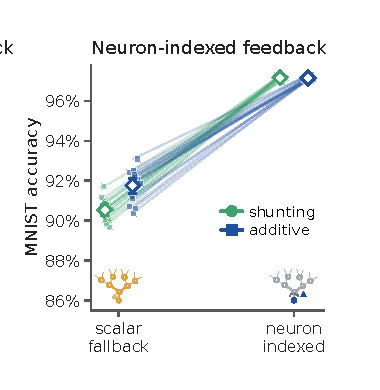
\includegraphics[width=\linewidth,height=3.45cm,keepaspectratio]{pdf_assets/identity_panel_b.pdf}\par
      \raggedright
      \headline[Add]{$7.8$--$11.2$ pp}{strict scalar $\rightarrow$
        neuron-specific feedback on MNIST}
    \end{column}
    \begin{column}{0.44\textwidth}
      \centering
      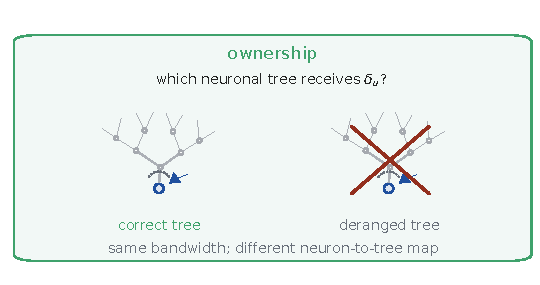
\includegraphics[width=\linewidth,height=1.50cm,keepaspectratio]{pdf_assets/ownership_schematic.pdf}\par
      \vspace{0.03cm}
      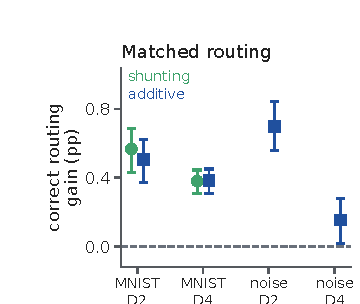
\includegraphics[width=0.82\linewidth,height=1.80cm,keepaspectratio]{pdf_assets/ownership_margin.pdf}\par
      {\scriptsize\color{Mute}same coordinates and bandwidth; only the
       neuron-to-tree assignment changes\par}
      \raggedright
      \vspace{0.06cm}
      {\large\bfseries\color{Add}$+0.15$ to $+0.70$ pp\par}
      {\scriptsize\color{Mute}correct ownership, favored in 58/60 paired comparisons\par}
    \end{column}
  \end{columns}
  \vfill
  \takeaway{The dominant bottleneck is neuron identity; routing inside the chosen neuron is a second, smaller problem on these tasks.}
  \vspace{0.04cm}
\end{frame}

% 16 — credit-conflict task and analytic boundary
\begin{frame}{Credit conflict creates demand for a branch address}
  \framesubtitle{Every branch gets a nonzero view; context selects the task-relevant one downstream.}
  \begin{columns}[T,onlytextwidth]
    \begin{column}{0.53\textwidth}
      \centering
      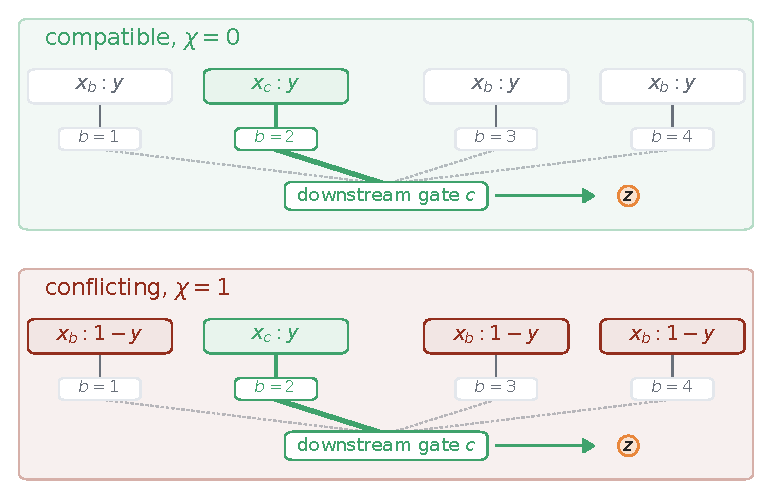
\includegraphics[width=\linewidth,height=4.52cm,keepaspectratio]
        {pdf_assets/path_necessity_task.pdf}\par
    \end{column}
    \begin{column}{0.43\textwidth}
      \deftag{conflict dose}\par
      {\footnotesize With probability $\chi$, every nonselected view carries the
       opposite class; otherwise it agrees.  The selector lies downstream of
       branch-local eligibility, so all $B$ local traces remain nonzero.\par}
      \vspace{0.07cm}
      \begin{columns}[T,totalwidth=\linewidth]
        \begin{column}{0.48\linewidth}
          {\scriptsize\color{Shunt}\bfseries correct path\par}
          {\small\color{Shunt}$\delta_b=\delta\mathbf 1[b=c]$\par}
        \end{column}
        \begin{column}{0.48\linewidth}
          {\scriptsize\color{Amber}\bfseries neuron shared\par}
          {\small\color{Amber}$\widetilde\delta_b=\delta/B$\par}
        \end{column}
      \end{columns}
      \vspace{0.08cm}
      \claimbox{\deftag{analytic boundary}\par
        \vspace{0.05cm}
        {\small
        \[
          C_{\chi}=(1-2\chi)\bm 1\bm 1^{\mathsf T}+2\chi I_B,
        \]
        \vspace{-0.22cm}
        \[
          \lambda_{\parallel}=B-2\chi(B-1),\qquad
          \chi_c(B)=\frac{B}{2(B-1)}.
        \]}}
    \end{column}
  \end{columns}
  \vfill
  \takeaway{This isolates a need for branch-selective information, not a dendrite-exclusive material implementation.}
  \vspace{0.04cm}
\end{frame}

% 17 — confirmatory path-necessity result
\begin{frame}{The path benefit appears at the predicted conflict boundary}
  \framesubtitle{Twenty confirmatory seeds; correct path, analytic backpropagation, and gated-point emulation coincide.}
  \begin{columns}[T,onlytextwidth]
    \begin{column}{0.73\textwidth}
      \centering
      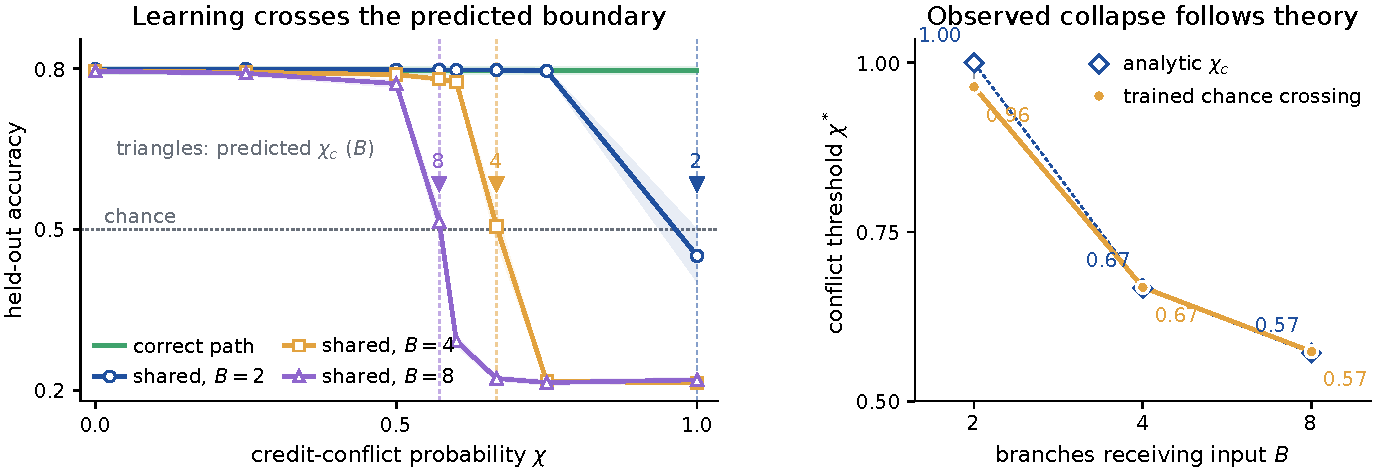
\includegraphics[width=\linewidth,height=4.72cm,keepaspectratio]
        {pdf_assets/path_necessity_results.pdf}\par
    \end{column}
    \begin{column}{0.23\textwidth}
      \vspace{0.03cm}
      \deftag{no conflict}\par
      {\footnotesize $\chi=0$: mean correct-minus-shared difference
       $\leq0.16$ percentage points.\par}
      \vspace{0.11cm}
      \headline[Shunt]{$+58.2$ pp}{correct path minus shared credit at
        $B=4$, $\chi=1$}
      \vspace{0.08cm}
      \deftag{ordered transition}\par
      {\large\bfseries $\chi^*_{8}<\chi^*_{4}<\chi^*_{2}$\par}
      {\scriptsize\color{Mute}utility and trained accuracy; 20/20 seeds\par}
    \end{column}
  \end{columns}
  \vfill
  \takeaway{Branch-selective credit pays only when nonselected branches carry conflicting evidence.}
  \vspace{0.04cm}
\end{frame}

% 18 — ancestry budget sweep
\begin{frame}{Ancestry routes help only at intermediate bandwidth}
  \framesubtitle{The benefit is consistent with an interior-bandwidth regime and disappears at full rank.}
  \begin{columns}[T,onlytextwidth]
    \begin{column}{0.40\textwidth}
      \centering
      \CreditTree[mode=address,K=4,scale=0.91,
        stagelabel={four nested ancestry routes}]
      \raggedright
      \headline[Dend]{$+1.27$ pp at $K=4$}{versus the best rank-matched
        non-anatomical route}
    \end{column}
    \begin{column}{0.56\textwidth}
      \centering
      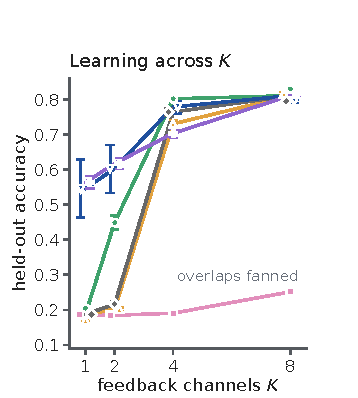
\includegraphics[width=\linewidth,height=5.20cm,keepaspectratio]{pdf_assets/subtree_k_sweep.pdf}\par
    \end{column}
  \end{columns}
  \vfill
  \takeaway{Anatomical ancestry is conditionally useful, not universally optimal.}
  \vspace{0.04cm}
\end{frame}

% 19 — physical depth
\begin{frame}{Physical depth helps only for task-matched serial computation}
  \framesubtitle{Depth is an inductive bias, not a free source of accuracy.}
  \begin{columns}[T,onlytextwidth]
    \begin{column}{0.48\textwidth}
      \centering
      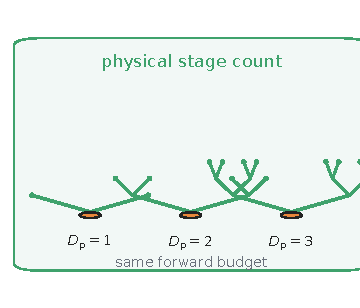
\includegraphics[width=\linewidth,height=2.10cm,keepaspectratio]{pdf_assets/physical_stage_schematic.pdf}\par
      \vspace{0.07cm}
      \eqstrip{V_n=\frac{E_n+C_n}{1+E_n+I_n+G_n+\epsilon}}
      \raggedright
      \headline[Shunt]{$+31$ pp}{aligned D3 minus D1 on a constructed
        multiplicative hierarchy, with branch units and parameters matched}
    \end{column}
    \begin{column}{0.48\textwidth}
      \centering
      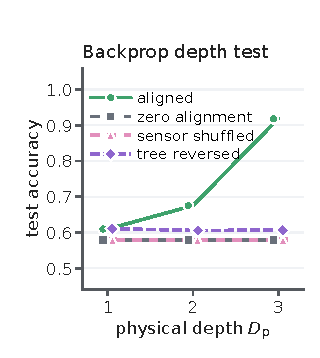
\includegraphics[width=\linewidth,height=3.85cm,keepaspectratio]{pdf_assets/physical_depth_headline.pdf}\par
      \vspace{0.06cm}
      {\scriptsize Independent sensors, shuffled sensors, and reversed order
       remain flat; at fixed budgets, depth per se reduced accuracy in 40/40
       seeds.\par}
    \end{column}
  \end{columns}
  \vfill
  \takeaway{Serial dendrites help only when the hierarchy of computation matches the hierarchy of the task.}
  \vspace{0.04cm}
\end{frame}

% 20 — reconstructed arbors
\begin{frame}{Reconstructed arbors provide sparse candidate routes}
  \framesubtitle{Morphology supplies capacity; it does not establish that endogenous learning uses it.}
  \begin{columns}[T,onlytextwidth]
    \begin{column}{0.40\textwidth}
      \centering
      \CreditTree[mode=address,K=8,scale=0.82,
        stagelabel={an ancestry dictionary with eight channels}]
      \vspace{0.05cm}
      \begin{columns}[T,totalwidth=\linewidth]
        \begin{column}{0.47\linewidth}
          {\fontsize{17}{19}\selectfont\bfseries\color{Shunt}$85\%$\par}
          {\fontsize{7}{8.4}\selectfont\color{Mute}dense-field capture at
            approximately 7\% of dense wiring\par}
        \end{column}
        \begin{column}{0.47\linewidth}
          {\fontsize{17}{19}\selectfont\bfseries\color{Violet}$2.7\times$\par}
          {\fontsize{7}{8.4}\selectfont\color{Mute}capture per connection
            beyond a density-matched shuffle\par}
        \end{column}
      \end{columns}
    \end{column}
    \begin{column}{0.56\textwidth}
      \centering
      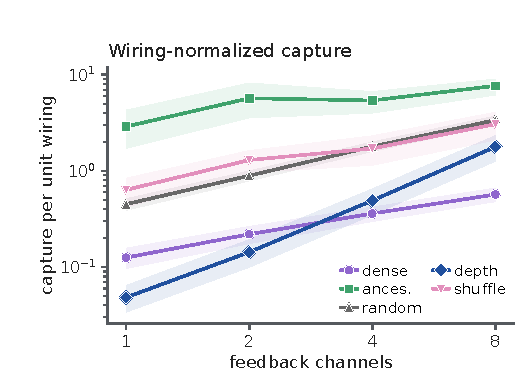
\includegraphics[width=\linewidth,height=3.80cm,keepaspectratio]{pdf_assets/capture_per_wire.pdf}\par
      {\scriptsize\color{Mute}Most of the gain is sparsity; morphology adds a
       bounded anatomy-specific margin.\par}
    \end{column}
  \end{columns}
  \vfill
  \takeaway{Real arbors are economical route dictionaries, but route availability is not evidence of route use.}
  \vspace{0.04cm}
\end{frame}

% 21 — focal shunting with boundary
\begin{frame}{Focal shunting changes descendant transport conditionally}
  \framesubtitle{The established result is transport selectivity, not a generic improvement in trained learning.}
  \begin{columns}[T,onlytextwidth]
    \begin{column}{0.37\textwidth}
      \centering
      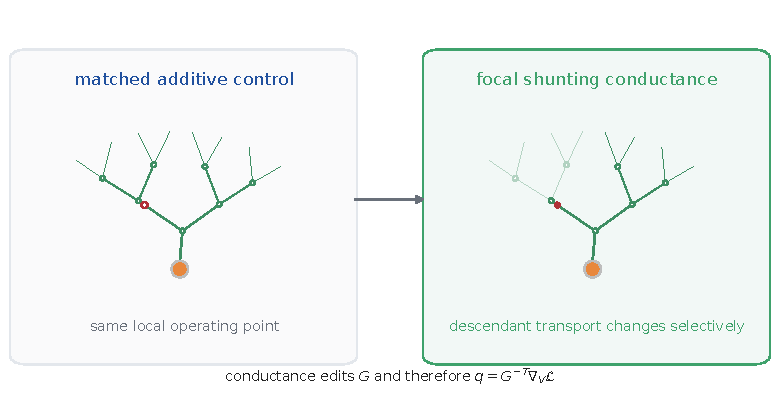
\includegraphics[width=\linewidth,height=2.25cm,keepaspectratio]{pdf_assets/focal_shunt_schematic.pdf}\par
      \vspace{0.06cm}
      \headline[Shunt]{$0.069$}{shunt-minus-additive localization contrast;
        matched local voltage, somatic state, and output error}
    \end{column}
    \begin{column}{0.31\textwidth}
      \centering
      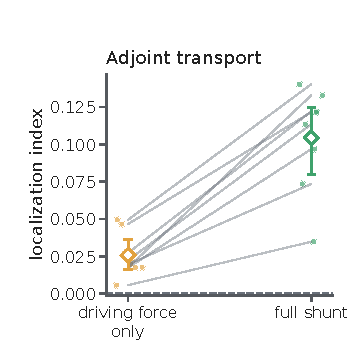
\includegraphics[width=\linewidth,height=3.55cm,keepaspectratio]{pdf_assets/transport_contrast_h.pdf}\par
      {\scriptsize\color{Mute}freezing the adjoint removes the contrast;
       restoring full transport recovers it\par}
    \end{column}
    \begin{column}{0.28\textwidth}
      \centering
      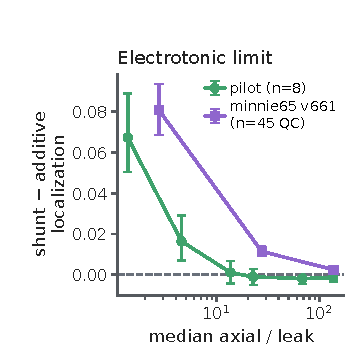
\includegraphics[width=\linewidth,height=3.05cm,keepaspectratio]{pdf_assets/focal_boundary.pdf}\par
      \vspace{0.08cm}
      \claimbox{\tiny Null at textbook resting calibration; present in
        high-conductance regimes. The exploratory adaptive-shunting study did
        not improve final loss over no shunt.\par}
    \end{column}
  \end{columns}
  \vfill
  \takeaway{Conductance can edit route gain locally, but this does not imply an unconditional learning advantage.}
  \vspace{0.04cm}
\end{frame}

% 22 — measured functional null
\begin{frame}{Measured responses show no morphology-specific alignment}
  \framesubtitle{Complete-tree visual-response credit is not better captured by ancestry routes than matched controls.}
  \begin{columns}[T,onlytextwidth]
    \begin{column}{0.30\textwidth}
      \centering
      \CreditTree[mode=address,K=4,scale=0.54,
        stagelabel={same arbor; competing dictionaries}]
      \vspace{0.08cm}
      {\fontsize{17}{19}\selectfont\bfseries\color{Mute}null\par}
      {\fontsize{7.5}{9}\selectfont\color{Mute}ancestry-minus-control
        intervals include zero\par}
    \end{column}
    \begin{column}{0.66\textwidth}
      \centering
      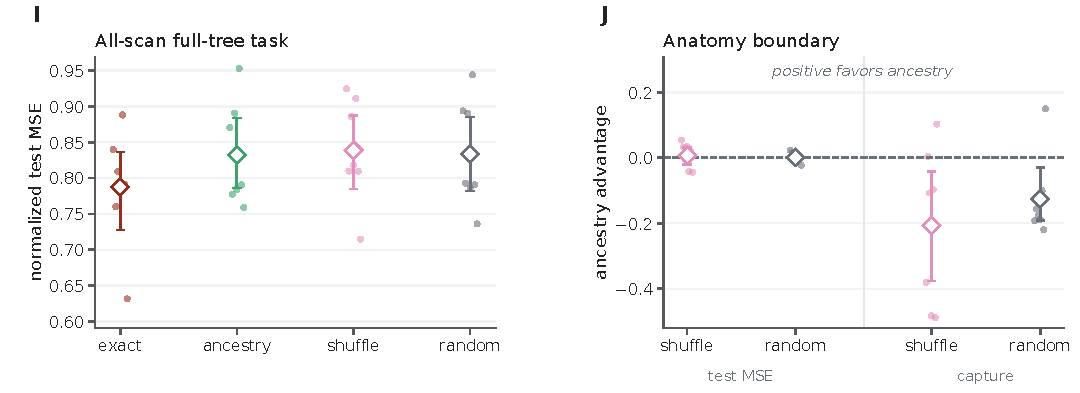
\includegraphics[width=\linewidth,height=4.10cm,keepaspectratio]{pdf_assets/fulltree_no_signed.pdf}\par
      {\scriptsize\color{Mute}Exact fields fit best; ancestry and matched
       low-rank controls remain statistically similar.\par}
    \end{column}
  \end{columns}
  \vfill
  \takeaway{Measured visual responses show no endogenous alignment with ancestry routes.}
  \vspace{0.04cm}
\end{frame}

% 23 — controlled alignment rescue
\begin{frame}{Task alignment rescues the same anatomical dictionary}
  \framesubtitle{Anatomy and channels stay fixed; only the task-gradient direction rotates.}
  \begin{columns}[T,onlytextwidth]
    \begin{column}{0.50\textwidth}
      \heroeq[alignment dose]{%
        \bm g(a)=\sqrt a\,\bm u_{\parallel}
          +\sqrt{1-a}\,\bm u_{\perp},
        \qquad \lVert QQ^{\mathsf T}\bm g(a)\rVert^2=a}
      \vspace{0.10cm}
      \headline[Violet]{$\rho_s=0.99$}{field capture predicts 20-step progress}
      \vspace{0.10cm}
      \claimbox{\footnotesize At $a=0$, nested routes lose to matched controls
        in 8/8 cells; at $a=1$, they win in 8/8.\par}
    \end{column}
    \begin{column}{0.46\textwidth}
      \centering
      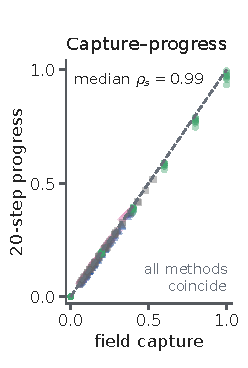
\includegraphics[width=\linewidth,height=4.20cm,keepaspectratio]{pdf_assets/alignment_rescue_n.pdf}\par
      {\scriptsize\color{Mute}Same cells, rank, gradient energy, and curvature;
       only alignment changes.\par}
    \end{column}
  \end{columns}
  \vfill
  \takeaway{Alignment can turn anatomical route capacity into a learning benefit.}
  \vspace{0.04cm}
\end{frame}

% 24 — external animal evidence
\begin{frame}{Animal learning is consistent with signed neuron coordinates}
  \framesubtitle{This is consistent with the first spatial rung; within-tree transport remains unmeasured.}
  \begin{columns}[T,onlytextwidth]
    \begin{column}{0.40\textwidth}
      \centering
      \vspace{0.16cm}
      \begin{tikzpicture}[line cap=round]
        \CTminitree{0}{0}
        \CTminitree{2.05}{0}
        \node[font=\scriptsize\bfseries,text=Shunt,anchor=north] at (0.02,-0.28) {P$^{+}$};
        \node[font=\scriptsize\bfseries,text=BP,anchor=north] at (2.07,-0.28) {P$^{-}$};
        \draw[Shunt,-{Stealth[length=4pt]},line width=1.0pt] (0.95,0.45)--(0.95,1.15);
        \draw[BP,-{Stealth[length=4pt]},line width=1.0pt] (3.00,1.15)--(3.00,0.45);
        \node[font=\tiny,text=Shunt,anchor=south] at (0.95,1.22) {$+$};
        \node[font=\tiny,text=BP,anchor=north] at (3.00,0.38) {$-$};
      \end{tikzpicture}
      \headline[Add]{$83.7\%$}{of contrast energy lies in the signed,
        neuron-specific mode; 6/6 animals}
      {\scriptsize\color{Mute}causal signs were fixed by the BCI mapping and
       predict opposite dendritic contrasts\par}
    \end{column}
    \begin{column}{0.56\textwidth}
      \centering
      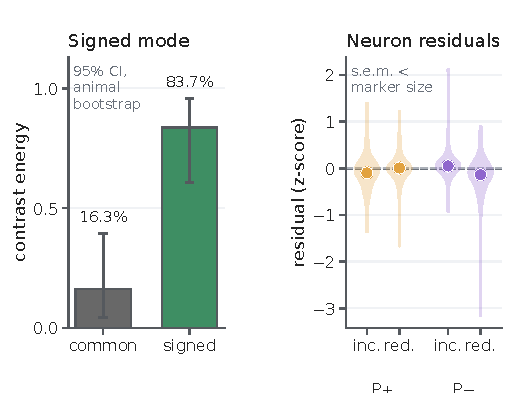
\includegraphics[width=\linewidth,height=4.75cm,keepaspectratio]{pdf_assets/animal_signed.pdf}\par
    \end{column}
  \end{columns}
  \vfill
  \takeaway{The animal result is consistent with signed neuron coordinates; routing within a tree remains open.}
  \vspace{0.04cm}
\end{frame}

% 25 — populated evidence plane
\begin{frame}{One phase plane organizes the positive and null results}
  \framesubtitle{Markers are measured or simulated outcomes; the background is the theory-guided regime map.}
  \centering
  \vspace{0.08cm}
  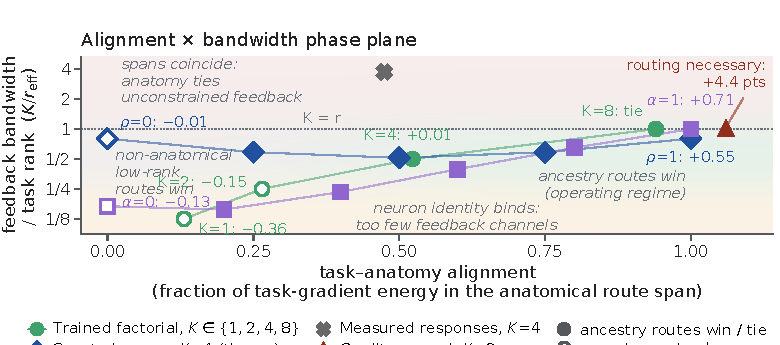
\includegraphics[width=0.96\linewidth,height=5.05cm,keepaspectratio]{pdf_assets/phase_plane.pdf}\par
  \vfill
  \takeaway{The same signal–noise theory explains where dendritic routes help and where they do not.}
  \vspace{0.04cm}
\end{frame}

% 26 — resource ledger, predictions and close
\begin{frame}{Dendrites change the resource ledger, not the exact ceiling}
  \framesubtitle{The contribution is structured local credit routing, conditional on alignment.}
  \begin{columns}[T,onlytextwidth]
    \begin{column}{0.31\textwidth}
      \deftag{exact ceiling}\par
      \vspace{0.08cm}
      {\footnotesize A point system given the same routed field matches the
       dendritic implementation. Exact backpropagation remains the
       first-order ceiling.\par}
      \vspace{0.16cm}
      \centering
      \CreditTree[mode=address,K=4,scale=0.39,
          stagelabel={same routed field}]\par
    \end{column}
    \begin{column}{0.34\textwidth}
      \deftag{what the tree contributes}\par
      \vspace{0.12cm}
      {\footnotesize\good{1.} local conductance state\par}
      \vspace{0.14cm}
      {\footnotesize\good{2.} reusable within-neuron addresses\par}
      \vspace{0.14cm}
      {\footnotesize\good{3.} branch-local route-gain control\par}
      \vspace{0.14cm}
      {\footnotesize\good{4.} sparse feedback wiring\par}
      \vspace{0.26cm}
      \headline[Shunt]{$85\%$ at $7\%$}{dense capture at a small fraction of dense wiring}
    \end{column}
    \begin{column}{0.31\textwidth}
      \deftag{decisive experiments}\par
      \vspace{0.12cm}
      {\footnotesize\textbullet\ focal inhibition should shift plasticity
       below the branch\par}
      \vspace{0.14cm}
      {\footnotesize\textbullet\ the shift should scale with dose and input
       resistance, then saturate\par}
      \vspace{0.14cm}
      {\footnotesize\textbullet\ useful routing should track task–route
       alignment, not morphology alone\par}
      \vspace{0.18cm}
      \centering
      \CreditTree[mode=shunt,shunted=true,scale=0.58,
        stagelabel={focal test of route gain}]
    \end{column}
  \end{columns}
  \vfill
  \takeaway{Coordinates select neurons; trees address synapses; conductance tunes route gain; alignment decides whether any of it pays.}
  \vspace{0.04cm}
\end{frame}


% ---- Backup divider + backup frames (always part of the single deck) ------
\appendix
\setbeamertemplate{footline}{%
  \leavevmode\hbox{%
    \begin{beamercolorbox}[wd=0.72\paperwidth,ht=0.30cm,dp=0.14cm,leftskip=0.7cm]{footline}%
      \color{Mute}\tiny Dendritic credit\enspace\textperiodcentered\enspace backup slides%
    \end{beamercolorbox}%
    \begin{beamercolorbox}[wd=0.28\paperwidth,ht=0.30cm,dp=0.14cm,rightskip=0.7cm]{footline}%
      \hfill\color{Mute}\tiny A\insertframenumber%
    \end{beamercolorbox}}%
}

% Backup divider: plain (no footline), matching the act-divider layout.
\begin{frame}[t,plain]
  \vspace{1.55cm}
  {\color{Shunt}\bfseries\scriptsize BACKUP\par}
  \vspace{0.30cm}
  {\fontsize{20}{25}\selectfont\bfseries\color{Ink}Derivations, controls, audits\par}
  \vspace{0.28cm}
  {\small\color{Mute}For questions\par}
  \vfill
  \hfill\stackmotif{4}\par
  \vspace{0.45cm}
\end{frame}
\setcounter{framenumber}{0}

% ---------------------------------------------------------------------------
% dendritic_credit_workshop_appendix.tex — backup slides (7 frames).
% The seven strongest backup frames kept in the single-deck build: adjoint
% chain, U(M) derivation + caveat, factorial control battery, validity /
% clean-agreement audit, reliability + same-span, CIFAR-10 confirmation,
% references. The five
% frames cut in the one-deck revision are preserved verbatim in the
% \iffalse block at the end of this file (nothing is lost).
% Backup frames keep the boxed \eqpanel look by design.
% ---------------------------------------------------------------------------

% A1 — adjoint chain
\begin{frame}{Appendix: the adjoint chain, from implicit function to path product}
  \begin{columns}[T,onlytextwidth]
    \begin{column}{0.55\textwidth}
      \eqpanel[general adjoint]{%
        \small
        \[
          \bm F(\bm V,\bm g,\bm x)=\bm 0,\qquad
          J_V=\frac{\partial\bm F}{\partial\bm V},\qquad
          J_V^{\mathsf T}\bm q=\nabla_{\bm V}\mathcal L
        \]
        \[
          \frac{\partial\mathcal L}{\partial g_i}
          =-\bm q^{\mathsf T}\frac{\partial\bm F}{\partial g_i}
          =x_i(E_i-V_n)\,q_n
        \]
        {\scriptsize\color{Mute}synapse-local factor $\times$ compartment
         adjoint\par}}
      {\footnotesize With the residual convention $\bm F=G\bm V-\bm b$.
       For the triangular tree system,
       $q_n=R_n^{\mathrm{tot}}\,\partial\mathcal L/\partial V_n$, so the
       adjoint and compartment factorizations are the same identity with the
       input-resistance factor moved between terms.\par}
    \end{column}
    \begin{column}{0.42\textwidth}
      {\footnotesize In a reciprocal passive cable, $J_V=G$ is symmetric
       positive definite and $G^{-\mathsf T}=G^{-1}$: the adjoint is a
       Green's-function solve. For a general nonsymmetric or recurrent
       compartmental system the inverse transpose is essential.\par
       \vspace{0.10cm}
       This fixed-point adjoint is the steady-state member of the
       Almeida--Pineda recurrent-backpropagation lineage.\par}
    \end{column}
  \end{columns}
  \vfill
  \takeaway{Credit is always eligibility times an adjoint; only the adjoint changes.}
  \vspace{0.04cm}
\end{frame}

% A2 — U(M) derivation
\begin{frame}{Appendix: deriving $U(M)$ and its exactness caveat}
  \begin{columns}[T,onlytextwidth]
    \begin{column}{0.55\textwidth}
      \eqpanel[descent lemma]{%
        \small For $L$-Lipschitz $\nabla\mathcal L$ and
        $\bm w^{+}=\bm w-\eta M\widehat{\bm g}$, $\widehat{\bm g}=\bm g+\bm\xi$:
        \[
          \begin{aligned}
            \E\,\mathcal L(\bm w^{+})\leq{}&\mathcal L(\bm w)
              -\eta\,\bm g^{\mathsf T}M\bm g\\
            &+\frac{L\eta^{2}}{2}
              \bigl(\lVert M\bm g\rVert_2^{2}+\tr(M\Sigma M^{\mathsf T})\bigr)
          \end{aligned}
        \]
        Optimizing the right side over $\eta$ when
        $\bm g^{\mathsf T}M\bm g>0$:
        \[
          U(M)=\frac{[\bm g^{\mathsf T}M\bm g]^{2}}
            {2L\bigl\{\lVert M\bm g\rVert_2^{2}
              +\tr(M\Sigma M^{\mathsf T})\bigr\}}
        \]}
    \end{column}
    \begin{column}{0.42\textwidth}
      {\footnotesize\deftag{caveat}\par
       The bound is an upper guarantee for a general $L$-smooth loss and is
       exact for the corresponding quadratic when curvature equals $L$ on the
       update directions; comparisons of $U(M)$ otherwise order guarantees,
       not necessarily realized losses.\par
       \vspace{0.10cm}
       Diagnostics: $U(M)$ predicted norm-matched one-step progress with
       Spearman $\rho=0.937$ and final held-out accuracy with $\rho=0.916$
       across 540 dendritic-route conditions; spectral capture alone
       predicted one-step progress at $\rho=0.877$.\par}
    \end{column}
  \end{columns}
  \vfill
  \takeaway{One-step geometry predicts within-family progress; trajectory-accrued advantages can escape it.}
  \vspace{0.04cm}
\end{frame}

% A3 — factorial control battery
\begin{frame}{Appendix: factorial control battery and implementation equivalence}
  \begin{columns}[T,onlytextwidth]
    \begin{column}{0.60\textwidth}
      \centering
      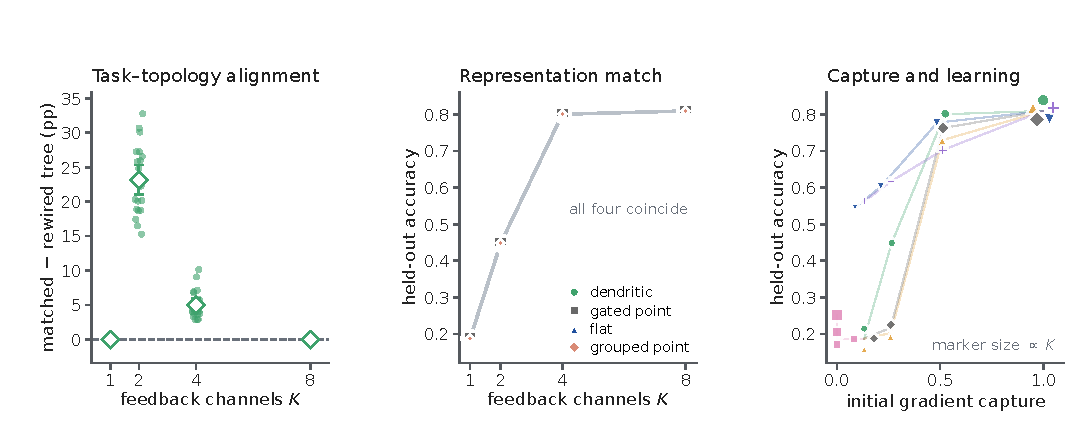
\includegraphics[width=\linewidth,height=4.30cm,keepaspectratio]{pdf_assets/factorial_controls_legend.pdf}
    \end{column}
    \begin{column}{0.36\textwidth}
      \footnotesize
      \deftag{topology alignment}\par matched tree minus rewired tree:
      $+0.231$ at $K{=}2$, $+0.050$ at $K{=}4$; 20/20 paired seeds each.\par
      \vspace{0.10cm}
      \deftag{representation match}\par dendritic, gated-point, flat and
      grouped-point implementations coincide exactly (maximum accuracy
      difference 0) when given identical routed fields.\par
      \vspace{0.10cm}
      \deftag{capture is not fate}\par fields with similar initial capture
      but different route signs and task alignment learned differently.\par
    \end{column}
  \end{columns}
  \vfill
  \takeaway{An address resource any point system can buy with the same routes.}
  \vspace{0.04cm}
\end{frame}

% A4 — validity audit + clean agreement
\begin{frame}{Appendix: input-validity audit and clean exact/BP agreement}
  \begin{columns}[T,onlytextwidth]
    \begin{column}{0.55\textwidth}
      \footnotesize
      \deftag{outcome-independent rule}\par signed synthetic drive is invalid
      for a positive-conductance shunting denominator: 640 signed-shunting
      runs are invalid, and the 400-run inhibitory-dose family that depends
      on them is excluded with its 200 valid partners --- 840 of 1,840 runs
      leave inference; all remain in the ledger.\par
      \vspace{0.10cm}
      \deftag{clean-source audit}\par all 320 detached clean-source runs
      passed the configuration, log, metric and checkpoint audit; synthetic
      shunting uses a non-negative transfer.\par
      \vspace{0.10cm}
      \deftag{agreement}\par all four depth-averaged exact-minus-BP intervals
      include zero; mean across 160 pairs $-0.055$ pp; largest single pair
      difference $5.90$ pp.\par
    \end{column}
    \begin{column}{0.41\textwidth}
      \centering
      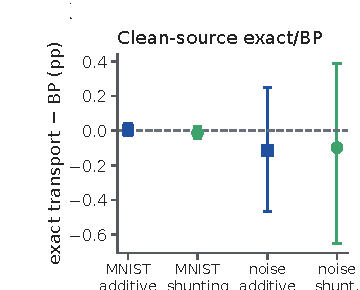
\includegraphics[width=\linewidth,height=3.55cm,keepaspectratio]{pdf_assets/clean_agreement.pdf}\par
      {\scriptsize\color{Mute}10 seeds $\times$ 4 depths $\times$ 2 tasks
       $\times$ 2 cores $\times$ 2 methods --- condition-average agreement,
       not pointwise identity\par}
    \end{column}
  \end{columns}
  \vfill
  \takeaway{The clean audit supports agreement on average, never formal equivalence.}
  \vspace{0.04cm}
\end{frame}

% A5 — reliability gain + same-span conditioning
\begin{frame}{Appendix: reliability gain, and same-span conditioning}
  \begin{columns}[T,onlytextwidth]
    \begin{column}{0.485\textwidth}
      \eqpanel[finite-step gain]{%
        \small For disjoint branches with signal $S_b$, noise $N_b$, step
        $\eta=c/L$:
        \[
          \mathcal G_c(\bm a)=\frac{c}{L}\sum_b
            \Bigl[a_bS_b-\frac{c\,a_b^{2}}{2}(S_b+N_b)\Bigr]
        \]
        \[
          a_b^{*}=\min\Bigl\{1,\frac{S_b}{c\,(S_b+N_b)}\Bigr\}
        \]}
      {\footnotesize A point model supplied with identical branch gates must
       match --- and did, to numerical precision.\par
       {\scriptsize\color{Mute}trained branch model, 50 fresh seeds: aligned
        shunting beat the best global gain by $0.001817$ in one-step loss
        reduction (49/50); final aligned-minus-no-shunt loss was null
        ($0.000425$, $P=0.154$)\par}}
    \end{column}
    \begin{column}{0.485\textwidth}
      \eqpanel[same-span field iteration]{%
        \small
        \[
          \bm f_{t+1}=\bm f_t-cA(\bm f_t-\bm g-\bm\xi_t)
        \]
        \[
          \E\,\mathcal L_T=\frac12\sum_j
            \Bigl[B_{j,T}+\frac{\sigma^{2}}{n}V_{j,T}\Bigr]
        \]}
      \centering
      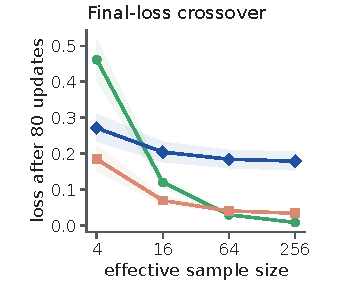
\includegraphics[height=2.00cm,keepaspectratio]{pdf_assets/same_span_crossover_e.pdf}\par
      {\scriptsize\color{Mute}\raggedright rank-eight same-span coordinates,
       condition numbers 1 / 15 / 388.5: slow modes filter noise at small
       $n$, orthogonal modes cut bias at large $n$; predicted crossovers
       $n^{*}=38.5$, $8.25$\par}
    \end{column}
  \end{columns}
  \vfill
  \takeaway{Conductance realizes the predicted ordering; conditioning trades bias against variance.}
  \vspace{0.04cm}
\end{frame}

% A6 — fresh CIFAR-10 confirmation
\begin{frame}{Appendix: harder data isolates the feedback bottleneck}
  \framesubtitle{Fresh 20-seed raw-additive confirmation; flattened CIFAR-10 is a transfer assay, not a vision benchmark.}
  \begin{columns}[T,onlytextwidth]
    \begin{column}{0.56\textwidth}
      \centering
      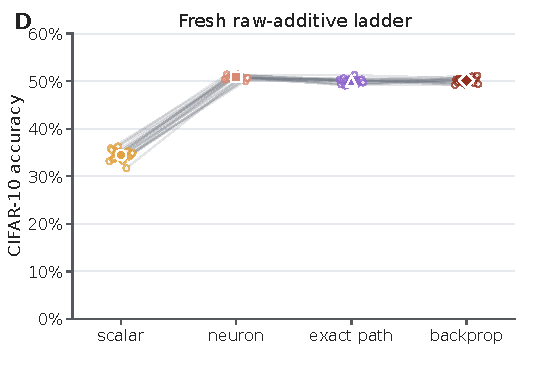
\includegraphics[width=\linewidth,height=4.75cm,keepaspectratio]{pdf_assets/cifar_confirmatory_ladder.pdf}\par
      {\scriptsize\color{Mute}Gray lines pair seeds; large symbols show means
       and 95\% intervals.\par}
    \end{column}
    \begin{column}{0.40\textwidth}
      \footnotesize
      \deftag{adequate control}\par matched BP: \(50.12\%\); all 80 fits passed
      source, calibration, checkpoint and convergence audits.\par
      \vspace{0.12cm}
      \deftag{neuron identity}\par \(+16.39\) pp over strict scalar
      (95\% CI 15.88--16.91; 20/20 seeds).\par
      \vspace{0.12cm}
      \deftag{path boundary}\par exact path was \(0.86\) pp below
      neuron-specific feedback; the prespecified path-resolution gate failed.\par
      \vspace{0.12cm}
      \deftag{implementation check}\par exact path was equivalent to matched BP
      within \(\pm1\) pp (TOST \(P=1.58\times10^{-5}\)).\par
    \end{column}
  \end{columns}
  \vfill
  \takeaway{Harder data magnifies neuron identity, not a generic benefit of finer dendritic transport.}
  \vspace{0.04cm}
\end{frame}

% A7 — references
\begin{frame}{Appendix: references}
  \vspace{0.05cm}
  \begin{columns}[T,onlytextwidth]
    \begin{column}{0.48\textwidth}
      % ragged right + tied journal~year units: no orphaned years
      {\color{Mute}\fontsize{7}{9}\selectfont\raggedright
       Rumelhart, Hinton \& Williams, \emph{Nature}~1986.\par
       Rall, dendritic cable theory, 1962.\par
       Almeida 1987; Pineda 1987 --- recurrent backpropagation.\par
       Werfel, Xie \& Seung, \emph{Neural Computation}~2005.\par
       Lillicrap, Cownden, Tweed \& Akerman, \emph{Nat.~Commun.}~2016.\par
       N\o kland, \emph{NeurIPS}~2016.\par
       Fr\'emaux \& Gerstner, \emph{Front.~Neural Circuits}~2016.\par
       Scellier \& Bengio, \emph{Front.~Comput.~Neurosci.}~2017.\par
       Whittington \& Bogacz, \emph{Neural Computation}~2017.\par
       Guerguiev, Lillicrap \& Richards, \emph{eLife}~2017.\par
       Sacramento, Costa, Bengio \& Senn, \emph{NeurIPS}~2018.\par
       Payeur, Guerguiev, Zenke, Richards \& Naud,
         \emph{Nat.~Neurosci.}~2021.\par
       Song et al., inferred-activity plasticity, 2024.\par}
    \end{column}
    \begin{column}{0.48\textwidth}
      {\color{Mute}\fontsize{7}{9}\selectfont\raggedright
       Holt \& Koch, shunting and firing rates, \emph{Neural Comput.}~1997.\par
       Chance, Abbott \& Reyes, gain modulation, \emph{Neuron}~2002.\par
       Destexhe, Rudolph \& Par\'e, high-conductance state,
         \emph{Nat.~Rev.~Neurosci.}~2003.\par
       Vogels et al., inhibitory plasticity, \emph{Science}~2011.\par
       Gidon \& Segev, spatial inhibitory domains, \emph{Neuron}~2012.\par
       Lovett-Barron et al., dendritic inhibition,
         \emph{Nat.~Neurosci.}~2012.\par
       Carandini \& Heeger, divisive normalization,
         \emph{Nat.~Rev.~Neurosci.}~2012.\par
       Jordan et al., conductance-based dendrites, 2024.\par
       MICrONS Consortium, \emph{Nature}~2025.\par
       Schneider-Mizell et al., inhibitory census, \emph{Nature}~2025.\par
       Ding et al., like-to-like wiring, \emph{Nature}~2025.\par
       Francioni et al., vectorized instructive signals,
         \emph{Nature}~2026.\par
       Safaai, Richards \& Sabatini, local credit manuscript, 2026.\par}
    \end{column}
  \end{columns}
  \vfill
  \takeaway{All quantitative claims trace to the journal manuscript and its source-data package.}
  \vspace{0.04cm}
\end{frame}

% ===========================================================================
% CUT FRAMES — preserved, not compiled.
% The five backup frames removed in the one-deck revision (former A2
% quotient-rule steps, A4 weighted projection / Ky--Fan, A5 reliability gain
% physical test, A6 Sherman--Morrison selectivity, A9 same-span
% bias--variance, A10 full-tree all-scan boundary; A5+A9 were merged into
% the kept "reliability + same-span" frame above). To restore one, move it
% above this block.
% ===========================================================================
\iffalse

% former A2 — quotient rule steps
\begin{frame}{Appendix: quotient-rule steps for eligibility}
  \begin{columns}[T,onlytextwidth]
    \begin{column}{0.52\textwidth}
      \eqpanel[synaptic conductance]{%
        \small With $V_n=N_n/G_n$,\quad
        $\partial_{g_i}N_n=x_iE_i$, \ $\partial_{g_i}G_n=x_i$:
        \[
          \begin{aligned}
            \partial_{g_i}V_n
            &=\partial_{g_i}\bigl(N_nG_n^{-1}\bigr)
             =x_iE_iG_n^{-1}-N_nG_n^{-2}x_i\\
            &=x_iG_n^{-1}\bigl(E_i-N_nG_n^{-1}\bigr)
             =x_iR_n^{\mathrm{tot}}(E_i-V_n)
          \end{aligned}
        \]}
    \end{column}
    \begin{column}{0.44\textwidth}
      \eqpanel[coupling conductance]{%
        \small The same algebra for a child coupling:
        \[
          \frac{\partial V_n}{\partial g^{\mathrm{den}}_{c\to n}}
          =R_n^{\mathrm{tot}}\bigl(f_c(V_c)-V_n\bigr)
        \]}
      {\footnotesize The driving-force form is exact for any conductance that
       enters both numerator and denominator. If $g_i=\psi(\theta_i)$, then
       $\partial_{\theta_i}\mathcal L
        =(\partial_{g_i}\mathcal L)\,\psi'(\theta_i)$.\par}
    \end{column}
  \end{columns}
  \vfill
  \takeaway{Every conductance parameter of the tree has a closed-form, synapse-local sensitivity.}
  \vspace{0.04cm}
\end{frame}

% former A4 — weighted projection and Ky-Fan
\begin{frame}{Appendix: weighted projection, covariance matching, Ky--Fan}
  \begin{columns}[T,onlytextwidth]
    \begin{column}{0.52\textwidth}
      \eqpanel[weighted projection]{%
        \small
        \[
          \bar{\bm w}=W^{-1/2}\bm w,\quad
          \bar{\bm g}=W^{1/2}\bm g,\quad
          \overline\Phi=W^{1/2}\Phi_{T,K}
        \]
        \[
          \bm z^{*}=\overline\Phi^{\dagger}\bar{\bm g},\qquad
          P_{\Phi}=\overline\Phi\,\overline\Phi^{\dagger},\qquad
          \mathcal C_K=\frac{\bar{\bm g}^{\mathsf T}P_{\Phi}\bar{\bm g}}
            {\bar{\bm g}^{\mathsf T}\bar{\bm g}}
        \]}
      \eqpanel[covariance matching]{%
        \small
        \[
          \frac{\E\lVert P_{\Phi}\bar{\bm g}\rVert^{2}}
               {\E\lVert\bar{\bm g}\rVert^{2}}
          =\frac{\tr(P_{\Phi}\overline C_g)}{\tr(\overline C_g)}
        \]
        {\scriptsize\color{Mute}$\overline C_g=\E[\bar{\bm g}\bar{\bm g}
         ^{\mathsf T}]$; $W{=}I$ recovers the unweighted form.\par}}
    \end{column}
    \begin{column}{0.44\textwidth}
      {\footnotesize By the Ky--Fan principle, the unconstrained rank-$K$
       upper bound is the span of the leading $K$ eigenvectors of $C_g$.\par
       \vspace{0.10cm}
       The $K$-route ancestry span equals the span of the $K$ coarsest
       tree-Haar modes, so anatomy attains the rank-$K$ bound exactly when the
       leading rank-$K$ eigenspace lies inside the laminar span; its shortfall
       for a general covariance is bounded by the leading-eigenspace energy
       outside that span.\par
       \vspace{0.10cm}
       At $\eta=1/L_W$, projected and full one-step descent guarantees differ
       by exactly the factor $\mathcal C_K$.\par}
    \end{column}
  \end{columns}
  \vfill
  \takeaway{A route basis is useful only insofar as task-gradient energy lies in its span.}
  \vspace{0.04cm}
\end{frame}

% former A5 — reliability gain
\begin{frame}{Appendix: the reliability gain $a_b^{*}$, and its physical test}
  \begin{columns}[T,onlytextwidth]
    \begin{column}{0.50\textwidth}
      \eqpanel[finite-step gain]{%
        \small For disjoint branches with signal $S_b$, noise $N_b$, step
        $\eta=c/L$:
        \[
          \mathcal G_c(\bm a)=\frac{c}{L}\sum_b
            \Bigl[a_bS_b-\frac{c\,a_b^{2}}{2}(S_b+N_b)\Bigr]
        \]
        \[
          a_b^{*}=\min\Bigl\{1,\frac{S_b}{c\,(S_b+N_b)}\Bigr\}
        \]}
      {\footnotesize The reliability factor $S_b/(S_b+N_b)$ is the special
       case $c=1$. A point model supplied with identical branch gates must
       match --- and did, to numerical precision.\par}
    \end{column}
    \begin{column}{0.46\textwidth}
      \centering
      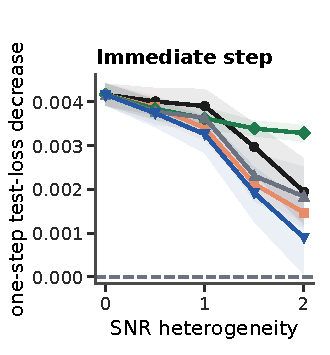
\includegraphics[height=3.15cm,keepaspectratio]{pdf_assets/reliability_step_c.pdf}\hspace{0.08cm}%
      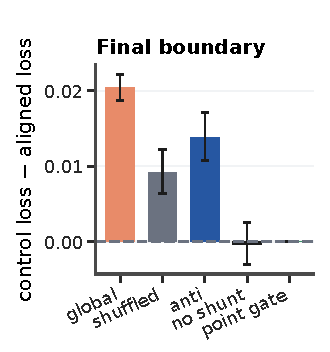
\includegraphics[height=3.15cm,keepaspectratio]{pdf_assets/reliability_final_f.pdf}\par
      \vspace{0.04cm}
      {\scriptsize\color{Mute}trained branch model, 50 fresh seeds: aligned
       shunting beat the best global gain by $0.001817$ in one-step loss
       reduction (49/50); final aligned-minus-no-shunt loss was null
       ($0.000425$, $P=0.154$)\par}
    \end{column}
  \end{columns}
  \vfill
  \takeaway{Conductance realizes the predicted ordering under a state clamp --- no more.}
  \vspace{0.04cm}
\end{frame}

% former A6 — Sherman-Morrison and selectivity
\begin{frame}{Appendix: Sherman--Morrison and electrotonic selectivity}
  \begin{columns}[T,onlytextwidth]
    \begin{column}{0.52\textwidth}
      \eqpanel[rank-one update]{%
        \small With $\bm q=G^{-1}\bm r$ and
        $G'=G+\kappa\,\bm e_k\bm e_k^{\mathsf T}$:
        \[
          (G+\kappa\,\bm e_k\bm e_k^{\mathsf T})^{-1}
          =G^{-1}-\frac{\kappa\,G^{-1}\bm e_k\bm e_k^{\mathsf T}G^{-1}}
            {1+\kappa\,\bm e_k^{\mathsf T}G^{-1}\bm e_k}
        \]
        \[
          \bm q'=\bm q-\frac{\kappa\,q_k}{1+\kappa\,(G^{-1})_{kk}}\,
            G^{-1}\bm e_k
        \]}
      {\footnotesize A current-matched additive perturbation changes $\bm b$
       but not $G$, so it cannot produce this adjoint update.\par}
    \end{column}
    \begin{column}{0.44\textwidth}
      \eqpanel[selectivity]{%
        \small With $\bm c_k=G^{-1}\bm e_k$, $r_k=(G^{-1})_{kk}$:
        \[
          \Delta\bm q=-a_k\bm c_k,\qquad
          |a_k|=\frac{\kappa_k|q_k|}{1+\kappa_kr_k}
        \]
        \[
          S_k=\frac{\operatorname{median}_{i\in D(k)}|c_{k,i}|}
                   {\operatorname{median}_{j\in C(k)}|c_{k,j}|}>1
        \]}
      {\footnotesize Dose sets amplitude (saturating at $|q_k|/r_k$); the
       Green's-function column sets spread. $S_k>1$ is necessary for
       descendant enrichment of absolute adjoint change, not sufficient for
       the full synaptic-gradient statistic.\par}
    \end{column}
  \end{columns}
  \vfill
  \takeaway{Input resistance controls dose response; axial and leak coupling control whether it is spatially selective.}
  \vspace{0.04cm}
\end{frame}

% former A9 — same-span bias-variance
\begin{frame}{Appendix: same-span conditioning trades bias against variance}
  \begin{columns}[T,onlytextwidth]
    \begin{column}{0.50\textwidth}
      \eqpanel[field iteration]{%
        \small
        \[
          \bm f_{t+1}=\bm f_t-cA(\bm f_t-\bm g-\bm\xi_t)
        \]
        For eigenmode $(\mu_j,\theta_j)$:
        \[
          \E\,\mathcal L_T=\frac12\sum_j
            \Bigl[B_{j,T}+\frac{\sigma^{2}}{n}V_{j,T}\Bigr]
        \]
        \[
          \begin{aligned}
            B_{j,T}&=(1-c\mu_j)^{2T}\theta_j^{2}\\
            V_{j,T}&=\frac{(c\mu_j)^{2}[1-(1-c\mu_j)^{2T}]}
              {1-(1-c\mu_j)^{2}}
          \end{aligned}
        \]}
    \end{column}
    \begin{column}{0.46\textwidth}
      \centering
      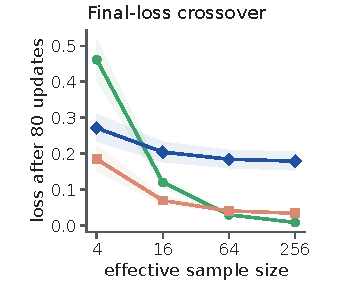
\includegraphics[height=2.85cm,keepaspectratio]{pdf_assets/same_span_crossover_e.pdf}\hspace{0.08cm}%
      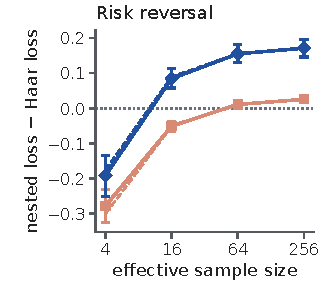
\includegraphics[height=2.85cm,keepaspectratio]{pdf_assets/same_span_risk_f.pdf}\par
      \vspace{0.04cm}
      {\scriptsize\color{Mute}three rank-eight same-span coordinates,
       condition numbers 1 / 15 / 388.5: slow modes filter noise at small
       $n$, orthogonal modes cut bias at large $n$; exact predicted median
       crossovers at $n^{*}=38.5$ and $8.25$\par}
    \end{column}
  \end{columns}
  \vfill
  \takeaway{Topology fixes capacity; conditioning trades bias against variance.}
  \vspace{0.04cm}
\end{frame}

% former A10 — full-tree all-scan boundary
\begin{frame}{Appendix: the full-tree all-scan boundary matches the predicted regime}
  \begin{columns}[T,onlytextwidth]
    \begin{column}{0.58\textwidth}
      \centering
      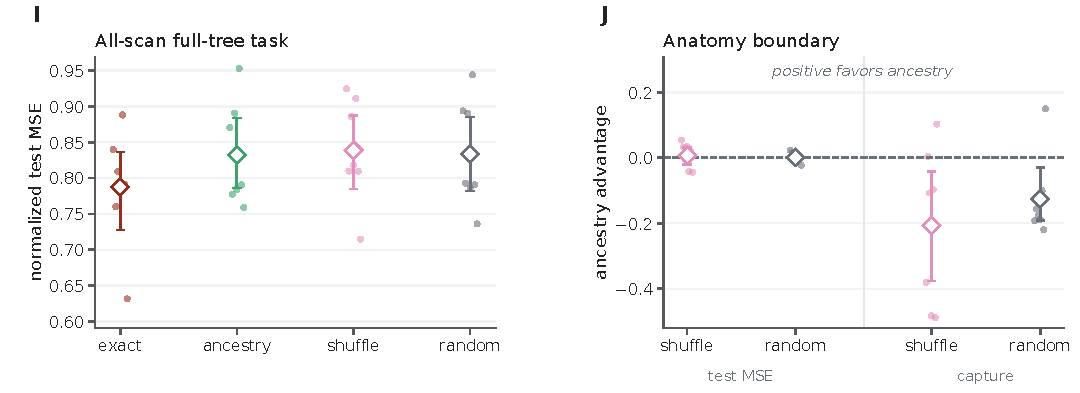
\includegraphics[width=\linewidth,height=3.90cm,keepaspectratio]{pdf_assets/fulltree_no_signed.pdf}
    \end{column}
    \begin{column}{0.38\textwidth}
      \footnotesize
      All 13 eligible scans, 520 method fits on complete reconstructed
      trees:\par
      \vspace{0.08cm}
      exact compartment error MSE \num{0.788}; topology $0.832$; random
      routes $0.833$; site-shuffled $0.839$ --- topology-minus-shuffle
      $0.0070$ $[-0.0207,0.0321]$: no reliable advantage.\par
      \vspace{0.08cm}
      In the coarse branch-surrogate family, a single channel already
      captured \num{0.965} of the measured response family's credit energy
      (effective rank 1.07), so every equal-rank dictionary spans it ---
      the regime where the credit-operator account predicts ties.\par
    \end{column}
  \end{columns}
  \vfill
  \takeaway{Rank-one task credit makes rank-matched dictionaries tie --- consistent with the predicted regime.}
  \vspace{0.04cm}
\end{frame}

\fi


\end{document}
